\chapter{Implémentation de la méthode linéaire dans Antares}

%Le plan du rapport doit être équilibré, c’est-à-dire que les paragraphes, à l’intérieur de chacune des deux parties principales (I. Présentation de l’entreprise, II. Présentation du travail réalisé) doivent être à peu près d’égale mesure. On évitera, par exemple, le mélange de paragraphes de 3 lignes avec d’autres de 60 lignes ; le rapport entre ces petits blocs de texte doit rester de 1 à 3.`

%– Le récit de l’expérience préprofessionnelle doit faire état de toutes les fonctions exercées par le stagiaire à son poste. Il doit comporter des développements techniques (illustrés par des schémas expliqués et commentés, par exemple), mais il s’agit avant tout de donner au lecteur une idée de ce que furent l’emploi du temps du stagiaire, ses tâches quotidiennes, les contraintes du métier, la nature des relations humaines dans cet environnement, les difficultés rencontrées et les résultats obtenus.
%– Les connaissances techniques acquises doivent transparaître dans le document. Le correcteur évaluera si celui-ci fait état d’une maîtrise réelle des outils (informatiques, mécaniques, etc.) utilisés pendant le stage. En outre, il estimera le niveau des connaissances techniques acquises que la rédaction du rapport aura su mettre en évidence.


Le stage a débuté au début du mois de juin 2024. Un ordinateur (mac équipé d'un processeur 2,3 GHz Intel Core i9 8 cœurs) et un PIN-pad générateur d'\ac{OTP} ont été mis à ma disposition. Des identifiants pour se connecter à un supercalculateur du CERFACS m'ont été donnés. Carlos, mon maître de stage, m'a fourni les informations nécessaires pour comprendre et utiliser Antares, une librairie de développement, à l'aide de la documentation en ligne\footnote{Documentation d'Antares : \href{https://cerfacs.fr/antares/}{cerfacs.fr/antares}}. Ensuite j'ai résolu un bug mineur sur Antares, ce qui m'a permis de me familiariser avec Nitrox, le Gitlab hébergé sur le serveur du CERFACS où sont situés Antares et d'autres codes du CERFACS.

Lors de mes essais sur le supercalculateur, j'ai utilisé une partition qui offre une puissance de calcul totale de 723 Tflop/s. Elle est composée de 185 nœuds Intel 2x18 cœurs Skylake, cadencés à 2,3 GHz avec 96 Go de mémoire. Ces ressources m'ont permis d'effectuer les tests demandant le plus de ressources.

\section{La librairie Antares}

Antares est une librairie Python/C++ développée depuis 2012 au CERFACS. Elle permet de traiter des données de simulation numérique issues de différents solveurs utilisés par le CERFACS et ses partenaires. Ces données sont organisées par Antares de manière unique et commune, ce qui est une grande force, notamment pour le partage et l'optimisation des post-traitements.
La bibliothèque inclut une cinquantaine de traitements, tels que la création de vues en coupe et l'interpolation.
Elle repose fortement sur la bibliothèque numpy pour tirer parti de ses algorithmes optimisés. %d'environ trois cents \ac{Mo}, composée de près de trois mille fichiers,
Chaque traitement est une classe composée d'une liste de mots-clefs qui correspondent à chaque paramètre. Certains sont nécessairement à donner par l'utilisateur, d'autres sont initialisés par défaut et peuvent être modifiés ou non. Nous retrouvons les deux paramètres 'source' et 'target' nécessaires au traitement d'interpolation ligne 3 et 4 de l'exemple de code \ref{lst:antares_2}. Les autres arguments du traitement d'interpolation sont listés plus bas (Tableau \ref{tab:arguments_interpolation1}).

Une solution CFD est interprétée par Antares comme une "Base".
Cette dernière peut être constituée d'une ou plusieurs zones.
Une zone représente un emplacement physique de la solution (par exemple, pour une chambre de combustion, nous pourrions avoir deux zones, régis avec des équations différentes: une avant les injecteurs et une après). % A vérifier par Carlos 
Chaque zone peut avoir un ou plusieurs instants.
Un instant est une "capture" de la solution à un instant t. Cela peut être la solution finale de la simulation par exemple. Plusieurs instants peuvent représenter une simulation dynamique, qui est utile dans le cas de l'aéroacoustique par exemple, où nous cherchons l'évolution temporelle de la pression.
Dans le cas où la structure du maillage ne change pas entre deux instants, Antares ne garde qu'une seule copie de la structure du maillage. Seules les variables changent entre les instants. On parle dans ce cas d'"instant partagé".\label{instants_partages}
% Généralement les instants sont identiques entre les zones, on dit qu'ils sont "partagés" tq les variables Carlos ?
Nous y retrouvons finalement les variables et leurs valeurs sur le maillage de la zone et instant en question.
% Ensuite chaque zone a un ou plusieurs instants où nous pouvons trouver la solution d'une variable, qui sera de même dimension que les coordonnées de l'instant.
La structure des solutions CFD interprétées dans Antares est illustrée ci-dessous (figure \ref{fig:structure_antares}):

\begin{figure}[H]
\centering
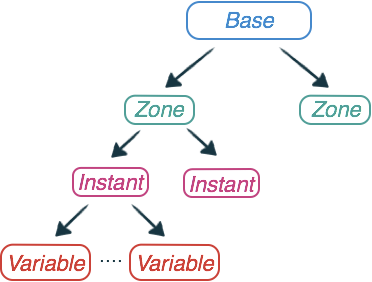
\includegraphics[width=0.42\textwidth]{images/data_structure_1.png}
\caption{Structure des données (source : \href{https://cerfacs.fr/antares/src/tutorial/base.html}{Antares tutorial})}
\label{fig:structure_antares}
%\footnote{Source:https://cerfacs.fr/antares/src/tutorial/base.html}
%\label{fig:https://cerfacs.fr/antares/src/tutorial/base.html}
\end{figure}

Voici un exemple d'utilisation d'Antares :

\begin{lstlisting}[caption=Exemple simple d'utilisation d'Antares (traitement d'interpolation), label={lst:antares_2}]
    import antares
    myt = antares.Treatment('interpolation')
    myt['source'] = source_base
    myt['target'] = target_base
    result = myt.execute()
\end{lstlisting}

Dans le cas ci-dessus, \texttt{result[0]} correspond à la première zone, \texttt{result[0][0]} à son premier instant et \texttt{result[0][0][0]} est un tableau numpy, manipulable par l'utilisateur, correspondant à la première variable du premier instant de la première zone.

Un point important pour l'interpolation linéaire est la connectivité (paragraph \ref{connectivité}). Si le maillage est non structuré, alors chaque cellule est définie par un type de forme et par ses sommets. Par exemple, elle peut être donnée par \texttt{base[0][0].connectivity['tri']} si la base contient des triangles (équivalent à avoir une connectivité "tri") dans sa zone 0 à l'instant 0.


\newpage
\section{Les différentes méthodes d'interpolation}

L'interpolation consiste à déterminer une fonction à partir d'un nombre fini de valeurs. En voici un exemple (Figure \ref{fig:interpolation_cloche_points}) en \ac{1D}. L'axe x représente la position et l'axe y la valeur des points.

\vspace{0,5cm}


\begin{figure}[H]
    \centering
    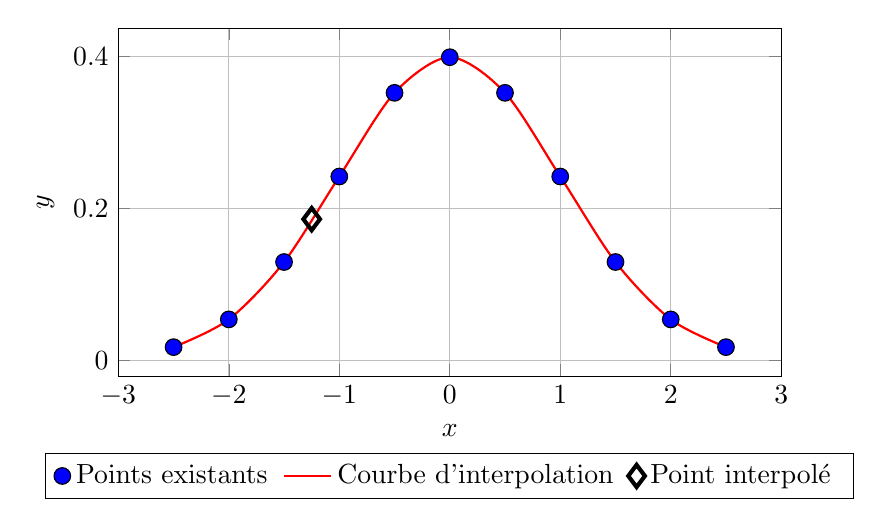
\begin{tikzpicture}
        \begin{axis}[
            width=10cm,
            height=6cm,
            xlabel={$x$},
            ylabel={$y$},
            grid=major,
            legend style={at={(0.5,-0.22)}, anchor=north, legend columns=-1},
        ]
    
        % Points existants (bleus) sur la courbe en cloche
        \addplot[
            only marks,
            mark=*,
            mark options={scale=1.5, fill=blue},
        ] coordinates {
            (-2.5, 0.0175)
            (-2, 0.05399)
            (-1.5, 0.1295)
            (-1, 0.24197)
            (-0.5, 0.35207)
            (0, 0.39894)
            (0.5, 0.35207)
            (1, 0.24197)
            (1.5, 0.1295)
            (2, 0.05399)
            (2.5, 0.0175)
        };        
        \addlegendentry{Points existants \hspace{0,3cm}}

        % Courbe rouge passant par les points
        \addplot[
            smooth,
            thick,
            red,
        ] coordinates {
            (-2.5, 0.0175)
            (-2, 0.05399)
            (-1.5, 0.1295)
            (-1, 0.24197)
            (-0.5, 0.35207)
            (0, 0.39894)
            (0.5, 0.35207)
            (1, 0.24197)
            (1.5, 0.1295)
            (2, 0.05399)
            (2.5, 0.0175)
        };
        \addlegendentry{Courbe d'interpolation \hspace{0,3cm}}
    
        % Point interpolé (vert)
        \addplot[
            only marks,
            mark=diamond,
            mark options={scale=2, fill=green, line width=1.5pt},
        ] coordinates {
            (-1.25, 0.1859)
            };
        \addlegendentry{Point interpolé \hspace{0,3cm}}
    
        \end{axis}
    \end{tikzpicture}
    \caption{Schéma d'interpolation avec des points sur une courbe en cloche}
    \label{fig:interpolation_cloche_points}
\end{figure}

Dans ce paragraphe, nous allons présenter les types d'interpolation \cite{cassiopee2015} implémentables dans Antares.
Cela implique certaines conditions, notamment sur le type de maillage.

Un maillage structuré est un maillage dont la connectivité\label{connectivité} entre les points peut être décrite de manière régulière, généralement à l'aide de tableaux multidimensionnels (1D, 2D, 3D). Dans un tel maillage, les points sont organisés en une grille régulière, ce qui permet de naviguer facilement à travers les données sans avoir à spécifier explicitement les relations entre les points.

En revanche, un maillage non-structuré est un maillage où les cellules ne peuvent pas être décrites de manière régulière. Elles sont définies par des formes géométriques quelconques où la connectivité des points ne suit pas un schéma régulier. Cela signifie que chaque cellule doit spécifier explicitement les points qui la composent, dans un ordre spécifique (\annexref{fig:ordre_connect}). Ces maillages sont souvent utilisés pour modéliser des géométries complexes où une grille régulière serait inadaptée.
%Voici le lien vers un site \cite{structure} qui explique la structure des cellules d'ordre supérieur, ce qui pourrait être utile pour l'implémentation d'une méthode d'ordre supérieur.

Dans Antares, nous visons principalement à traiter des maillages non structurés, car ils sont couramment utilisés dans les simulations modernes en raison de leur flexibilité à représenter des géométries complexes. Une autre condition est que la méthode d'interpolation doit être applicable en 1D, 2D et 3D. Un facteur à prendre en compte dans la méthode que l'on souhaite implémenter est aussi le temps de calcul, appelé 'coût'.

La caractérisation mathématique des fonctions à interpoler est un paramètre à prendre en compte. Cependant, les équations dont sont issues les solutions numériques en entrée dans Antares sont difficiles à caractériser mathématiquement (tel que l'équation de Naviers-Stokes) et le niveau en mathématiques est trop élevé pour pouvoir se plonger sur ce problème \cite{gordont1971_2}. C'est pour cela qu'il y aura peu de résultats mathématiques à présenter dans cette partie.
Ces méthodes ont déjà été implémentées et testées pour d'autres codes de simulation numérique, ce qui permet de nous donner idée de la qualité des résultats que nous pouvons espérer en fonction de la méthode d'interpolation.

\newpage

La plupart des méthodes d'interpolation simples peuvent s'écrire sous la forme

\begin{equation}
    \hat{f}(x) = \sum_{i=1}^{M} w_i(x) \cdot f(x_i)
\end{equation}


où :

- \(\hat{f}(x)\) est la valeur interpolée à la position \(x\),

\vspace{-0,2cm}

- \(f(x_i)\) est la valeur connue aux points de données \(x_i\) (ou une combinaison de valeurs de points connus),

\vspace{-0,2cm}

- \(w_i(x)\) est le poids associé à \(f(x_i)\),

\vspace{-0,2cm}

- \(M\) est le nombre total de points de données utilisés pour l'interpolation.

%\addcontentsline{toc}{section}{L'interpolation et l'aéroacoustique}



\subsection{La méthode par voisin le plus proche}
Cette première méthode est simple : nous prenons comme valeur \( v \) d'interpolation au point \( p \) la valeur \( v \) du point le plus proche de \( p \).
En voici quelques illustrations :

%\vspace{0.5cm}

\begin{figure}[H]
    \centering
        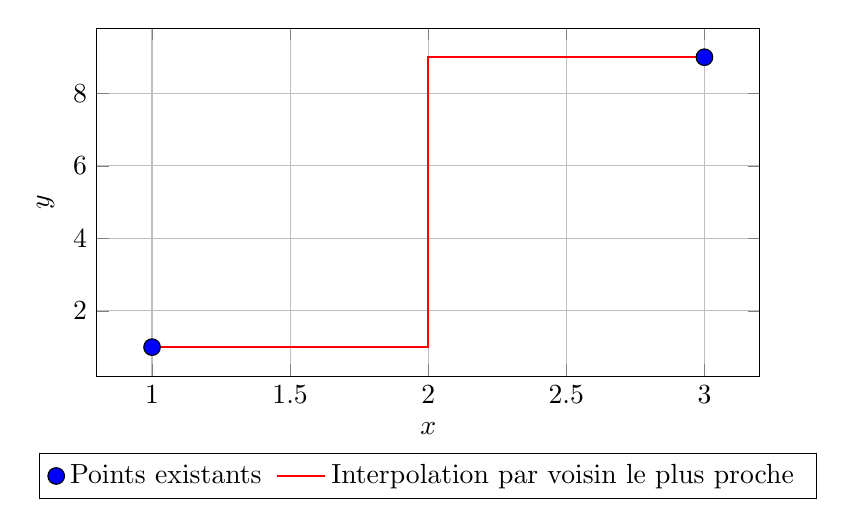
\begin{tikzpicture}
            \begin{axis}[
                width=10cm,
                height=6cm,
                xlabel={$x$},
                ylabel={$y$},
                grid=major,
                legend style={at={(0.5,-0.22)}, anchor=north, legend columns=-1},
            ]

            \addplot[
                only marks,
                mark=*,
                mark options={scale=1.5, fill=blue},
            ] coordinates {
                (1, 1)
                (3, 9)
            };
            \addlegendentry{Points existants \hspace{0,3cm}}

            \addplot[
                thick,
                red,
            ] coordinates {
                (1, 1)
                (2, 1)
                (2, 9)
                (3, 9)
            };
            \addlegendentry{Interpolation par voisin le plus proche \hspace{0,3cm}}

            %\addplot[
            %    only marks,
            %    mark=*,
            %    mark options={scale=1.5, fill=green},
            %] coordinates {
            %    (1.7, 1)
            %};
            %\addlegendentry{Point interpolé}

            \end{axis}
        \end{tikzpicture}
    \caption{Schéma d'interpolation par voisin le plus proche}
    \label{fig:interpolation_voisin}
\end{figure}

La courbe rouge représente l'interpolation sur tout le domaine x entre les deux points. Cela représente les coordonnées (x, y) de tous les potentiels points d'interpolation.
Cette méthode est discontinue et peu précise pour la plupart des fonctions.



\subsection{La méthode pondération inverse à la distance (IDW)}\label{sIDW} % déjà '\ac' 

La méthode IDW est aussi une méthode d'interpolation simple après la méthode du voisin le plus proche, toujours dans notre cas d'application. C'était la seule implémentée dans Antares (elle inclut aussi la méthode du voisin le plus proche comme expliqué plus tard dans cette section). Elle a pour formule :

\begin{equation}
    \hat{f}(x) = 
    \begin{cases}
    \frac{\sum_{i=1}^{M} \frac{f(x_i)}{d(x, x_i)^p}}{\sum_{i=1}^{M} \frac{1}{d(x, x_i)^p}}, & \text{si } d(x, x_i) \neq 0 \text{ pour tout } i, \\ 
    f(x_j), & \text{si } d(x, x_j) = 0 \text{ pour certains } j.
    \end{cases}
\end{equation}


\[
\text{avec} \quad w_i(\mathbf{x}) = \frac{1}{d(\mathbf{x}, \mathbf{x}_i)^p}
\]


où :

- \(\hat{f}(x)\) est la valeur interpolée à la position \(x\),

\vspace{-0,2 cm}

- \(f(x_i)\) est la valeur connue aux points de données \(x_i\),

\vspace{-0,2 cm}

- \(d(x, x_i)\) est la distance entre \(x\) et \(x_i\),

\vspace{-0,2 cm}

- \(p\) est le paramètre de puissance,

\vspace{-0,2 cm}

- \(M\) est le nombre total de points de données.


En voici des illustrations 1D :

\begin{figure}[H]
    \centering
    \begin{minipage}{0.45\textwidth}
        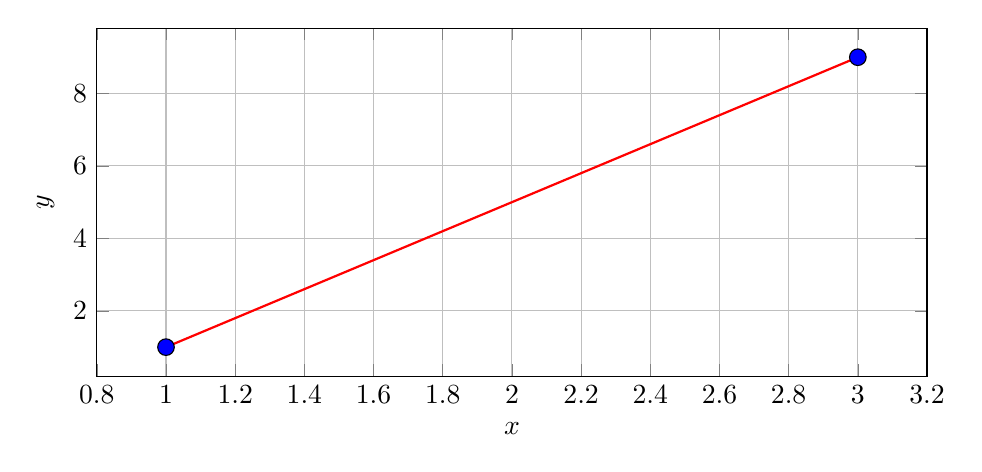
\begin{tikzpicture}
            \begin{axis}[
                width=\textwidth,
                height=6cm,
                xlabel={$x$},
                ylabel={$y$},
                grid=major,
            ]
            \addplot[
                only marks,
                mark=*,
                mark options={scale=1.5, fill=blue},
            ] coordinates {
                (1, 1)
                (3, 9)
            };

            \addplot[
                domain=1:3,
                samples=100,
                smooth,
                thick,
                red,
            ] {(1/abs(1-x) + 9/abs(x-3))/(1/(abs(1-x))+1/(abs(x-3)))};

            %\addplot[
            %    only marks,
            %    mark=*,
            %    mark options={scale=1.5, fill=green},
            %] coordinates {
            %    (2, 5)
            %};
            \end{axis}
        \end{tikzpicture}
        \caption{interpolation IDW M=2, p=1}
    \end{minipage}
    \hspace{0.5cm}
    \begin{minipage}{0.45\textwidth}
        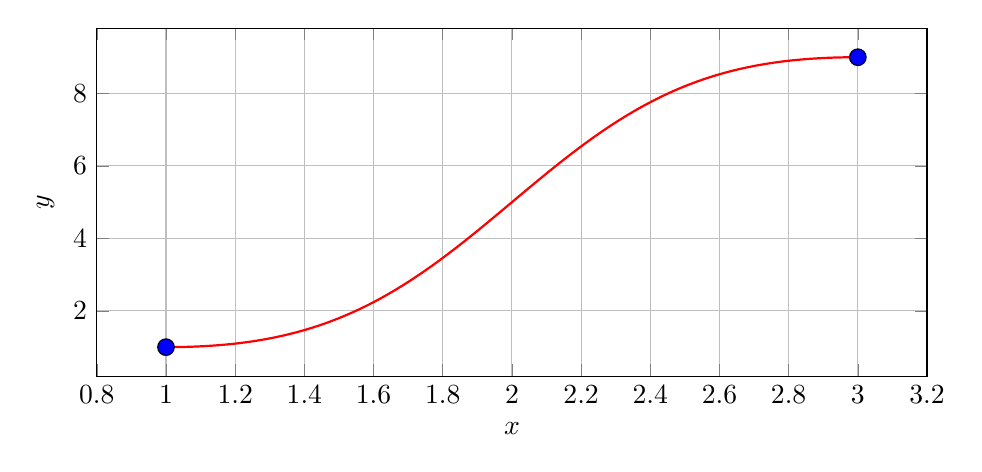
\begin{tikzpicture}
            \begin{axis}[
                width=\textwidth,
                height=6cm,
                xlabel={$x$},
                ylabel={$y$},
                grid=major,
            ]
            \addplot[
                only marks,
                mark=*,
                mark options={scale=1.5, fill=blue},
            ] coordinates {
                (1, 1)
                (3, 9)
            };

            \addplot[
                domain=1:3,
                samples=100,
                smooth,
                thick,
                red,
            ] {(1/(abs(1-x)^2) + 9/(abs(x-3)^2))/(1/(abs(1-x)^2)+1/(abs(x-3)^2))};

            %\addplot[
            %    only marks,
            %    mark=*,
            %    mark options={scale=1.5, fill=green},
            %] coordinates {
            %    (2, 5)
            %};
            \end{axis}
        \end{tikzpicture}
        \caption{interpolation IDW M=2, p=2}
    \end{minipage}

    \vspace{0.8cm}

    \begin{minipage}{0.45\textwidth}
        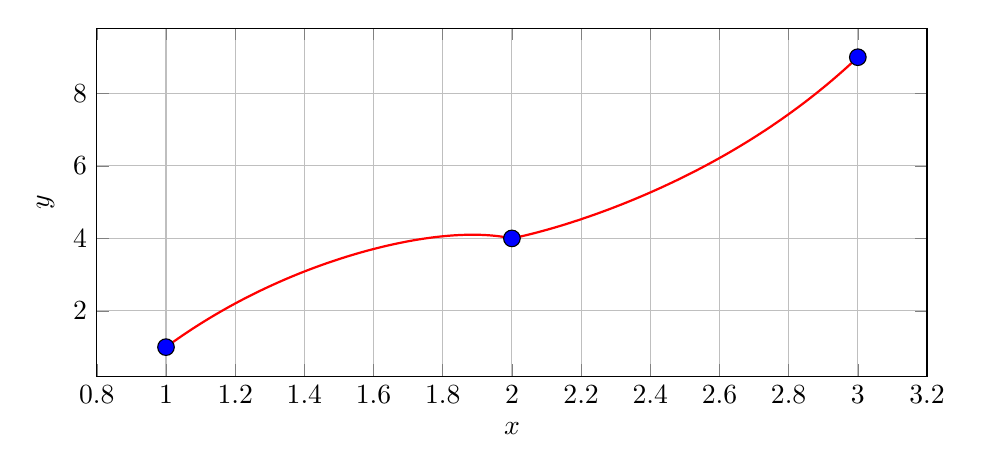
\begin{tikzpicture}
            \begin{axis}[
                width=\textwidth,
                height=6cm,
                xlabel={$x$},
                ylabel={$y$},
                grid=major,
            ]
            \addplot[
                only marks,
                mark=*,
                mark options={scale=1.5, fill=blue},
            ] coordinates {
                (1, 1)
                (3, 9)
                (2, 4)
            };

            \addplot[
                domain=1:3,
                samples=100,
                smooth,
                thick,
                red,
            ] {(1/abs(1-x) + 9/abs(x-3) + 4/abs(2-x))/(1/(abs(1-x)) + 1/(abs(x-3)) + 1/(abs(2-x)))};

            %\addplot[
            %    only marks,
            %    mark=*,
            %    mark options={scale=1.5, fill=green},
            %] coordinates {
            %    (1.5, 3.43)
            %};
            \end{axis}
        \end{tikzpicture}
        \caption{interpolation IDW M=3, p=1}
    \end{minipage}
    \hspace{0.5cm}
    \begin{minipage}{0.45\textwidth}
        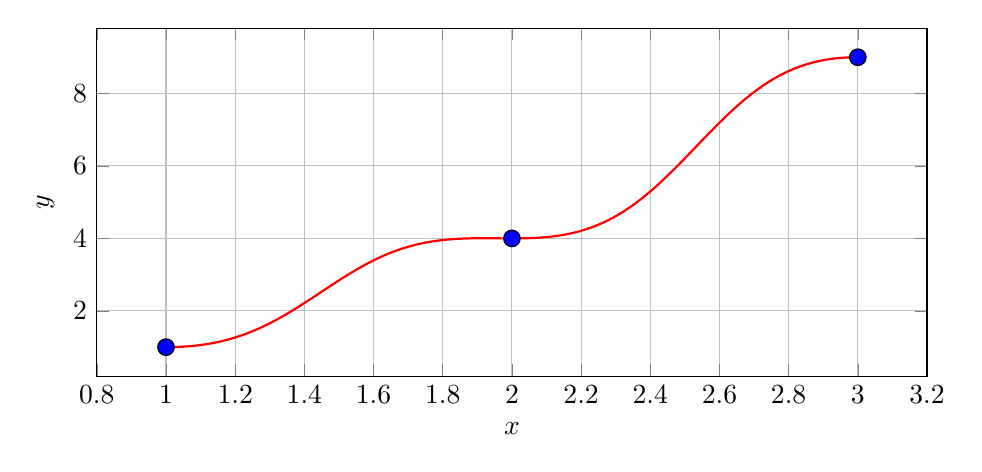
\begin{tikzpicture}
            \begin{axis}[
                width=\textwidth,
                height=6cm,
                xlabel={$x$},
                ylabel={$y$},
                grid=major,
            ]
            \addplot[
                only marks,
                mark=*,
                mark options={scale=1.5, fill=blue},
            ] coordinates {
                (1, 1)
                (3, 9)
                (2, 4)
            };

            \addplot[
                domain=1:3,
                samples=100,
                smooth,
                thick,
                red,
            ] {(1/(abs(1-x)^2) + 9/(abs(x-3)^2) + 4/(abs(2-x)^2))/(1/(abs(1-x)^2) + 1/(abs(x-3)^2) + 1/(abs(2-x)^2))};

            %\addplot[
            %    only marks,
            %    mark=*,
            %    mark options={scale=1.5, fill=green},
            %] coordinates {
            %    (1.5, 2.84)
            %};
            \end{axis}
        \end{tikzpicture}
        \caption{interpolation IDW M=3, p=2}
    \end{minipage}
\end{figure}


\vspace{-0.5cm}

\begin{figure}[H]
    \centering
    
\includegraphics[width=0.39\textwidth]{images/legende-interp3.png}
\end{figure}


Dans notre cas, nous ne prenons pas en compte tous les \(M\) points du maillage source. Nous nous limitons à un nombre \(N\) de points les plus proches. 
Nous remarquons que pour \( N = 1 \), nous retrouvons la méthode du voisin le plus proche, pour tout \( p \).
Et pour \( N = 2 \) et \( p = 1 \), toujours en 1D, nous retrouvons la méthode linéaire.
Limiter le nombre de points dans le calcul implique une discontinuité lorsque nous changeons de point. Pour illustrer cela, voici une figure 1D (Figure \ref{fig:interpolation_IDW_1D_rayon}) où tous les points sont espacés d'une unité (seuls trois points sont représentés). Avec \(M = 5\) et \(N = 3\), cela revient ici à changer, loin des bords, l'un des trois points de calcul pour une valeur de \(x\) égale à un demi modulo un. Le modulo un est représenté par une ligne en pointillés noirs.%Il est appelé rayon, car en 2D, il est représenté par un cercle et en 3D pas une sphère. 


\begin{figure}[H]
    \centering
        \begin{tikzpicture}
            \begin{axis}[
                width=15cm,
                height=7cm,
                title={Interpolation IDW (M=5, N=3, p=2)},%, "rayon"=1)},
                xlabel={$x$},
                ylabel={$y$},
                grid=major,
                legend style={at={(0.5,-0.22)}, anchor=north, legend columns=-1},
            ]
            \addplot[
                only marks,
                mark=*,
                mark options={scale=1.5, fill=blue},
            ] coordinates {
                (1, 1)
                (2, 4)
                (3, 9)
                (4, 16)
                (5, 25)
            };
            \addlegendentry{Points existants\phantom{---}}
        
            % Plotting the radius for the nearest neighbors
            \addplot[dashed, aurometalsaurus, thick] coordinates {(2.5, 0) (2.5, 25)};
            \addlegendentry{Rayon de 1\phantom{---}}
        
            \addplot[
                domain=1:1.5,
                samples=100,
                smooth,
                thick,
                red,
            ] {(1/(abs(1-x)^2) + 9/(abs(x-3)^2) + 4/(abs(2-x)^2))/(1/(abs(1-x)^2) + 1/(abs(x-3)^2) + 1/(abs(2-x)^2))};
            \addplot[
                domain=1.5:2.5,
                samples=100,
                smooth,
                thick,
                red,
            ] {(1/(abs(1-x)^2) + 9/(abs(x-3)^2) + 4/(abs(2-x)^2))/(1/(abs(1-x)^2) + 1/(abs(x-3)^2) + 1/(abs(2-x)^2))};
            \addplot[
                domain=2.5:3.5,
                samples=100,
                smooth,
                thick,
                red,
            ] {(4/(abs(x-2)^2) + 9/(abs(3-x)^2) + 16/(abs(4-x)^2))/(1/(abs(x-2)^2) + 1/(abs(3-x)^2) + 1/(abs(4-x)^2))};
            \addplot[
                domain=3.5:4.5,
                samples=100,
                smooth,
                thick,
                red,
            ] {(9/(abs(x-3)^2) + 16/(abs(4-x)^2) + 25/(abs(5-x)^2))/(1/(abs(x-3)^2) + 1/(abs(4-x)^2) + 1/(abs(5-x)^2))};
            \addplot[
                domain=4.5:5,
                samples=100,
                smooth,
                thick,
                red,
            ] {(9/(abs(x-3)^2) + 16/(abs(4-x)^2) + 25/(abs(5-x)^2))/(1/(abs(x-3)^2) + 1/(abs(4-x)^2) + 1/(abs(5-x)^2))};
            \addlegendentry{Interpolation IDW}
        
            %\addplot[dashed, aurometalsaurus, thick] coordinates {(2.5, 0) (2.5, 25)};
            \addplot[dashed, aurometalsaurus, thick] coordinates {(3.5, 0) (3.5, 25)};
            %\addplot[dashed, aurometalsaurus, thick] coordinates {(4.5, 0) (4.5, 25)};
        
            \end{axis}
        \end{tikzpicture}
        \caption{Schéma d'interpolation IDW avec \(N\)=3}
        \label{fig:interpolation_IDW_1D_rayon}
\end{figure}
    

Nous observons une discontinuité en 2,5 et 3,5. La discontinuité peut être un grand problème pour la stabilité des schémas numériques.

\begin{comment}
    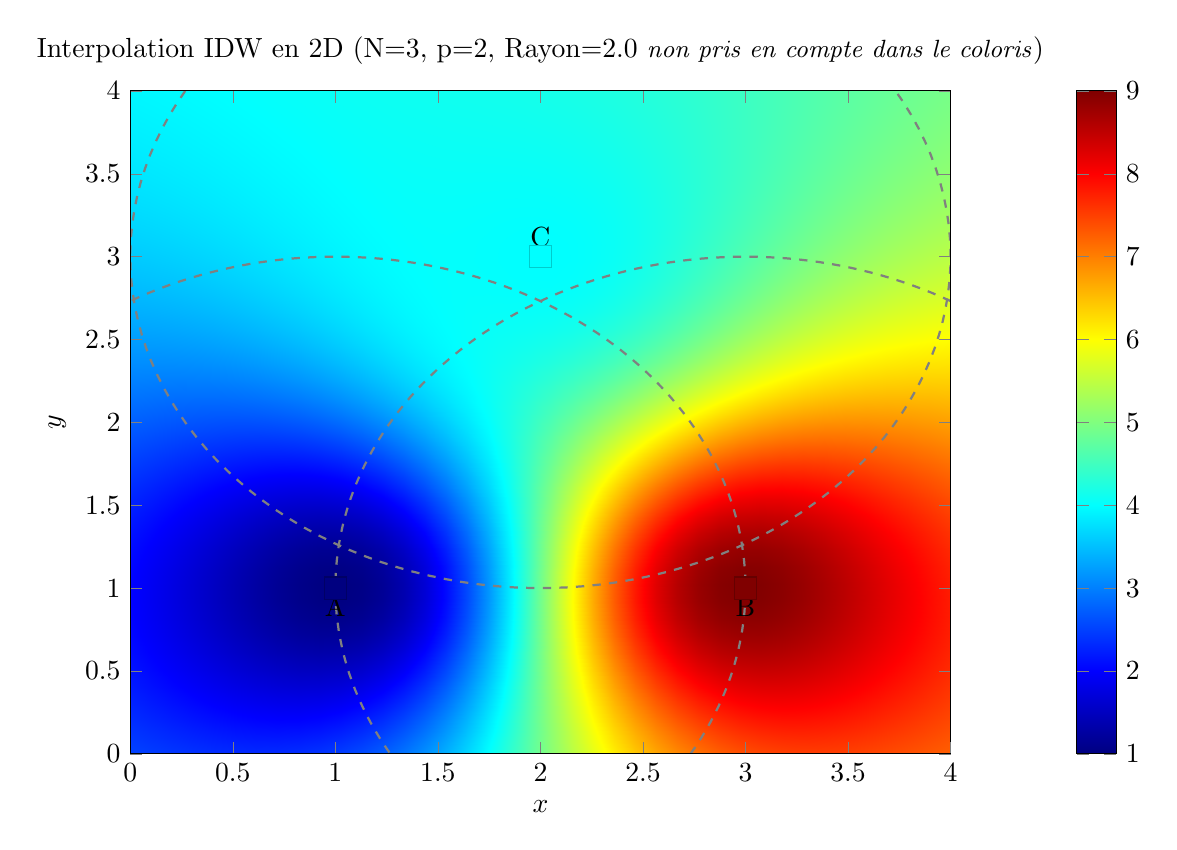
\begin{tikzpicture}
        \begin{axis}[
            view={0}{90},
            xlabel={$x$},
            ylabel={$y$},
            colorbar,
            title={Interpolation IDW en 2D (N=3, p=2, Rayon=2.0 {\small \textit{non pris en compte dans le coloris}})},
            colormap/jet,  % Utilisation d'une colormap standard
            width=12cm,
            height=10cm,
        ]

        % Points d'interpolation connus
        \pgfplotstableread{
            x y z
            1 1 1
            3 1 9
            2 3 4
        }\datatable

        % Fonction IDW
        \addplot3[
            surf,
            shader=interp,
            domain=0:4,
            y domain=0:4,
            samples=40,    % A augementer avant la version finale
        ] 
        {(1/(sqrt((x-1)^2+(y-1)^2 + 1e-6)^2) + 
        9/(sqrt((x-3)^2+(y-1)^2 + 1e-6)^2) + 
        4/(sqrt((x-2)^2+(y-3)^2 + 1e-6)^2)) / 
        (1/(sqrt((x-1)^2+(y-1)^2 + 1e-6)^2) + 
        1/(sqrt((x-3)^2+(y-1)^2 + 1e-6)^2) + 
        1/(sqrt((x-2)^2+(y-3)^2 + 1e-6)^2))};
        
        % Points d'interpolation connus
        \addplot3[
            only marks,
            scatter,
            scatter src=explicit,
            point meta=\thisrow{z},
            mark=square*,
            mark options={scale=2},
        ] table [x=x, y=y, z=z] {\datatable};

        % Tracer les cercles de rayon 2
        \addplot[
            draw=gray, 
            thick, 
            dashed, 
            domain=-30:120,
            samples=100,
        ] 
        ({1 + 2*cos(x)}, {1 + 2*sin(x)});  % Cercle autour du point A (1,1)

        \addplot[
            draw=gray, 
            thick, 
            dashed, 
            domain=60:210,
            samples=100,
        ] 
        ({3 + 2*cos(x)}, {1 + 2*sin(x)});  % Cercle autour du point B (3,1)

        \addplot[
            draw=gray, 
            thick, 
            dashed, 
            domain=-210:30,
            samples=100,
        ] 
        ({2 + 2*cos(x)}, {3 + 2*sin(x)});  % Cercle autour du point C (2,3)

        % Annoter les points
        \node at (axis cs:1,1,1) [anchor=north] {A};
        \node at (axis cs:3,1,9) [anchor=north] {B};
        \node at (axis cs:2,3,4) [anchor=south] {C};

        \end{axis}
    \end{tikzpicture}
\end{comment}

Nous pouvons aussi imaginer que 2 points, A et B, à droite et à gauche de 3 points (les plus proches) alignés selon la verticale, prendront la même valeur pour \( N \) = 3 :

\begin{figure}[H]
    \centering
    \begin{tikzpicture}

        % Les points sur la ligne verticale
        \filldraw[blue] (0, -1.2) circle (2pt) node[right] {$c$}; 
        \filldraw[blue] (0, 0) circle (2pt) node[right] {$b$};
        \filldraw[blue] (0, 1.5) circle (2pt) node[right] {$a$};
        
        % Les autres
        \filldraw[blue] (-4.7, -0.5) circle (2pt) node[above left] {$d$};
        \filldraw[blue] (5.2, 1.0) circle (2pt) node[above right] {$e$};
    
        % Les points à gauche et à droite qui prennent la même valeur
        \filldraw[red] (-1.5, 0.5) circle (2pt) node[above left] {A}; 
        \filldraw[red] (1.5, 0.5) circle (2pt) node[above right] {B};
    
        % Lignes de liaison entre les points rouges et les trois plus proches voisins
        \draw[dashed, gray] (-1.5, 0.5) -- (0, -1.2);
        \draw[dashed, gray] (-1.5, 0.5) -- (0, 0);
        \draw[dashed, gray] (-1.5, 0.5) -- (0, 1.5);
    
        \draw[dashed, gray] (1.5, 0.5) -- (0, -1.2);
        \draw[dashed, gray] (1.5, 0.5) -- (0, 0);
        \draw[dashed, gray] (1.5, 0.5) -- (0, 1.5);
    
    \end{tikzpicture}
    
    \caption{Schéma montrant la non-directivité d'IDW}
    %\label{fig:interpolation_IDW_rayon}
\end{figure}

    
Ce qui n'est pas cohérent dans le cas où le gradient selon l'horizontal n'est pas nul.
\begin{comment}
Un des problèmes avec la méthode IDW est que « \textit{a directional bias to the database solutions can shift the interpolated results} »\footnote{Traduction : « un biais directionnel dans les solutions de la base de données peut décaler les résultats interpolés. » Source : \textit{Titre de l'article}, Auteur, Année, URL si applicable.}.
\end{comment}
Un des problèmes avec la méthode IDW est qu'un biais directionnel dans les solutions de la base source peut décaler les résultats interpolés \cite{palmer2009, idw-mapscaping}.
Lorsque toutes les informations selon un axe de l'espace ne se situent que d'un côté, le gradient ne sera pas pris en compte et l'erreur sera élevée. Par exemple, cela est généralement le cas lorsque le maillage cible a des points qui se situent à l’extérieur du maillage source.
Cependant, il serait envisageable, dans certains cas, d'adopter des solutions alternatives, telles qu'en 2D, sélectionner trois points sources situés autour du point cible et répartis sur un angle supérieur à 180° \cite{idw-update}.  % \footnote{Traduction de : « \textit{One issue with the IDW method is that a directional bias to the database solutions can shift the interpolated results.} »


D'autres méthodes dérivées ou similaires existent pour évaluer nos poids (les poids sont les distances inverses à la puissance \(p\) dans notre cas). La plus intéressante serait celle dite de Franke-Littke. Elle consiste à utiliser une distance maximale autour du point au-delà de laquelle les autres points ne sont pas pris en compte. Autrement dit, on utilise un cercle (dans le cas 2D) d'un certain rayon pour déterminer quels points nous sont utiles pour l'interpolation. Dans ce cas, le nombre de points est variable.
J'ai considéré subjectivement que cette méthode n'était pas intéressante. La méthode confrontée à un maillage ayant une différence de raffinement intrinsèque importante ne prendrait aucun point à certains endroits et dans d'autres lieux, un trop grand nombre de points devrait être calculé.

\begin{comment}
    Certaines conditions de cette méthode doivent être respectés, comme Pour N tends vers l’infini, p doit être inférieur ou égale à la dimension, par ex 3 pour ne pas diverger. Mais N n’est pas grand dans notre cas.
    Voir d'autres choses page 7 de mon ppt.
\end{comment}


%Une des limitation \cite{idw-mapscaping} de la méthode IDW est qu'elle n'a pas d'autocorrélation spatiale, contrairement à la méthode kriging qui sera décrite plus tard. 

\vspace{0,5 cm}


\newpage
\subsection{D'autres méthodes}\label{s223}
%\paragraph{1. La méthode polynomiale}
%\phantom{-}
%\newline
%L'interpolation polynomiale est d'un degré correspondant à celui du polynôme utilisé. Elle peut être réalisée en N dimensions sur un maillage structuré. Cette interpolation est de classe \(C^\infty\) (c'est-à-dire infiniment dérivable, avec des dérivées de tous ordres continues). Elle peut aussi être appliquée à des maillages non structurés, une méthode souvent utilisée au CERFACS est d'ajouter des points fictifs sur les arêtes des cellules % Sourcer la thèse d'Alexis

\subparagraph{a. Interpolation de Lagrange \cite{Barycentric_Lagrange1, Barycentric_Lagrange2}}
\textit{Type : Polynomiale} \\
\phantom{----}L'interpolation de Lagrange utilise un polynôme unique qui passe par \(n\) points donnés. Elle peut devenir imprécise pour un grand nombre de points à cause de l'effet Runge. Sa généralisation en 2D et 3D la rend coûteuse. La formule de Lagrange est donnée par :
\begin{equation}
    L(x) = \sum_{i=0}^{n} y_i \prod_{\substack{0 \leq j \leq n \\ j \neq i}} \frac{x - x_j}{x_i - x_j}
\end{equation}


%L'interpolation de Lagrange utilise un polynôme unique qui passe par tous les points donnés. Elle est souvent utilisée pour l'interpolation d'un petit nombre de points, mais elle peut devenir imprécise pour un grand nombre de points à cause de l'effet Runge. Il faut donc limiter le nombre de points (comme dans les méthodes déjà implémentées dans Antares).
%Nous pouvons retrouver sur un site \cite{structure} la structure des cellules pour de l'interpolation d'ordre supérieur (notamment pour Lagrange). Un inconvénient de cette méthode est que sa généralisation en 2D et surtout 3D est complexe.
%Une interpolation de Lagrange serait possible en partant de la méthode barycentrique. \cite{Barycentric_Lagrange1} \cite{Barycentric_Lagrange2}


%\subparagraph{b. Hermite \cite{bajaj}}
\subparagraph{b. Interpolation d'Hermite \cite{bajaj}}
\textit{Type : Polynomiale} \\
\phantom{----}L'interpolation d'Hermite est une extension de l'interpolation de Lagrange, prenant en compte non seulement les valeurs des points, mais aussi leurs dérivées. Pour cela, il faut reprendre le polynôme de Lagrange et imposer la continuité des dérivées. Cela permet de créer un polynôme d'interpolation plus lisse. Cependant, elle est coûteuse, surtout lorsqu'elle est étendue aux ordres supérieurs. La formule de l'interpolation d'Hermite est donnée par :
\begin{equation}
    H(x) = \sum_{i=0}^{n} \left[ y_i h_i(x) + y'_i h'_i(x) \right]
\end{equation}
où \( h_i(x) \) et \( h'_i(x) \) sont des fonctions de base Hermite.

%L'interpolation d'Hermite est une extension de l'interpolation, de Lagrange prend en compte non seulement les valeurs des points, mais aussi leurs dérivées. Cela permet de créer un polynôme d'interpolation plus lisse. Cependant, elle est coûteuse, surtout lorsqu'elle est étendue aux ordres supérieurs.

\subparagraph{c. Interpolation quadratique \cite{alexis}}
\textit{Type : Polynomiale} \\
\phantom{----}L'interpolation quadratique est une méthode qui utilise des polynômes de degré deux pour calculer des valeurs intermédiaires entre les points de données.
La forme simple de la formule 1D de l'interpolation quadratique pour un ensemble de trois points \( (x_0, y_0), (x_1, y_1), (x_2, y_2) \) est donnée par :

\vspace{-0,3 cm}

\begin{equation}
    f(x) = a_0 + a_1(x - x_1) + a_2(x - x_1)^2
\end{equation}

où les coefficients \( a_0, a_1, a_2 \) sont déterminés par les valeurs en \( x_0, x_1, x_2 \).

Dans le cas des maillages non-structurés en 2D ou 3D, l'interpolation quadratique peut être étendue à une forme plus générale. Par exemple, pour un maillage non-structuré en 2D, la formule peut être écrite comme ceci :

\vspace{-0,5 cm}

\begin{equation}
    f(x, y) = a_0 + a_1(x - x_1) + a_2(y - y_1) + a_3(x - x_1)^2 + a_4(y - y_1)^2 + a_5(x - x_1)(y - y_1)
\end{equation}

Une méthode applicable dans notre cas est décrite dans une thèse menée au CERFACS\cite{alexis}.


\subparagraph{d. Interpolation cubique \cite{tanaka}}
\textit{Type : Polynomiale} \\
\phantom{----}L'interpolation cubique est une méthode qui utilise des polynômes de degré trois pour calculer des valeurs intermédiaires entre les points de données. Cette méthode est souvent un bon compromis entre complexité et précision et pourrait être un bon candidat pour la prochaine méthode à implémenter. L'interpolation cubique peut être réalisée en utilisant soit des polynômes de Lagrange, soit des splines cubiques, soit un algorithme de convolution cubique.
La formule 1D de l'interpolation cubique entre quatre points \( x_0, x_1, x_2, x_3 \) est donnée par :

\vspace{-0,5 cm}

\begin{equation}
    f(x) = a_0 + a_1(x - x_1) + a_2(x - x_1)^2 + a_3(x - x_1)^3
\end{equation}

où les coefficients \( a_0, a_1, a_2, a_3 \) sont déterminés par les valeurs et les dérivées en \( x_0, x_1, x_2, x_3 \).
%Dans le contexte des maillages non réguliers, il serait pertinent d'explorer l'implémentation de l'interpolation tricubique.

%L'interpolation cubique est une méthode simple qui utilise des polynômes de degré trois pour calculer des valeurs intermédiaires entre les points de données.  Ce serait potentiellement le meilleur candidat pour la prochaine méthode à implémenter. %On pourrait alors utiliser le traitement gradient avec l'argument \texttt{vtk = True} pour avoir le gradient au nœud et non au centre de la cellule. Ensuite, dans le meilleur des cas, il faudrait simplement reprendre la fonction d'interpolation linéaire et mettre à jour le code "computes\_barycenters.py".
%"L'interpolation bicubique peut être accomplie en utilisant soit des polynômes de Lagrange, soit des splines cubiques, soit un algorithme de convolution cubique." (Wikipédia, Interpolation bicubique). Dans notre cas, il faudrait aussi implémenter l'interpolation tricubique, et ce, sur des maillages non réguliers.

\subparagraph{e. Splines cubiques \cite{gordont1971}}
\textit{Type : Polynomiale} \\
\phantom{----}Les splines cubiques sont une méthode d'interpolation qui utilise des polynômes de degré trois, ajustés de manière à garantir la continuité des premières et deuxièmes dérivées. Cela assure une transition lisse entre les segments de la courbe. Les splines sont stables et précises, notamment lorsqu'il est nécessaire de respecter certaines conditions aux frontières.

La formule 1D pour une spline cubique entre deux points \( x_i \) et \( x_{i+1} \) est donnée par :

\vspace{-0,5 cm}

\begin{equation}
    S_i(x) = a_i + b_i(x - x_i) + c_i(x - x_i)^2 + d_i(x - x_i)^3
\end{equation}

où les coefficients \( a_i, b_i, c_i, d_i \) sont déterminés de manière à ce que les fonctions soient continues, ainsi que leurs premières et deuxièmes dérivées, aux points de jonction.

Dans le cas de plusieurs segments, les splines cubiques forment une courbe composée de ces polynômes, ajustée de manière à minimiser la courbure totale tout en passant par tous les points de données.


\subparagraph{f. NURBS \cite{surface, piegl1995nurbs}}
\textit{Type : Polynomiale} \\
\phantom{----}Les \ac{NURBS} pourrait être un bon candidat pour l'interpolation. C'est une généralisation des splines, permettant de représenter des formes géométriques simples comme complexes. Elles sont notamment utilisées en CAO et pour l'interpolation de surfaces.
La formule 1D pour une courbe NURBS est :

\vspace{-0,6 cm}

\begin{equation}
    C(u) = \frac{\sum_{i=0}^{n} N_{i,p}(u) \cdot w_i \cdot P_i}{\sum_{i=0}^{n} N_{i,p}(u) \cdot w_i}
\end{equation}

\vspace{-0,4 cm}

où :

- \( C(u) \) : est la courbe NURBS paramétrée par \( u \).

\vspace{-0,2 cm}

- \( N_{i,p}(u) \) : est la base de la spline B-spline de degré \( p \) associée au nœud \( i \).

\vspace{-0,2 cm}

- \( w_i \) : est le poids associé au point de contrôle \( P_i \).

\vspace{-0,2 cm}

- \( P_i \) : est le point de contrôle correspondant.

\begin{comment}
    \paragraph{2. Méthodes à base de distance}
    \phantom{-}
    \newline
    Ces méthodes utilisent la distance entre les points de données pour calculer les valeurs interpolées, souvent en pondérant les contributions des points voisins.

Voici un tableau (Tableau \ref{tab:interpolation_methods}), donné dans une présentation de la NASA \cite{nasa}, donnant les différentes méthodes d'interpolation disponibles dans MATLAB en fonction des dimensions des données d'entré :
\begin{table}[ht]
    \centering
    \begin{tabular}{|l|c|c|c|}
    \hline
    \textbf{Méthode d'interpolation} & \textbf{Source 1D} & \textbf{Source 2D} & \textbf{Source 3D} \\ \hline
    Voisin le plus proche & X & X & X \\ \hline
    Linéaire & X & X & X \\ \hline
    Spline cubique & X & X & X \\ \hline
    Hermite cubique par morceaux & X & & \\ \hline
    Cubique & X & structuré uniquement & structuré uniquement \\ \hline % \phantom{-}
    Cubique utilisée dans MATLAB v5 & X & & \\ \hline
    \end{tabular}
    \caption{Tableau des méthodes d'interpolation en fonction des dimensions}
    \label{tab:interpolation_methods}
\end{table}
\end{comment}

%\subsection{L'interpolation par Splines}

%\paragraph{2. Méthodes géostatistiques}
%\phantom{-}
%\newline



\subparagraph{g. Kriging \cite{palmer2009, kringing}}
\textit{Type : Géostatistique} \\
\phantom{----}Définissons deux termes utiles pour caractériser la méthode suivante :

- Autocorrélation spaciale : Mesure du degré auquel les données sont agglomérées ou désordonnées dans l'espace. Voici une application d'autocorrelation (filtre gaussien) sur des données :
\begin{figure}[H]
    \centering
    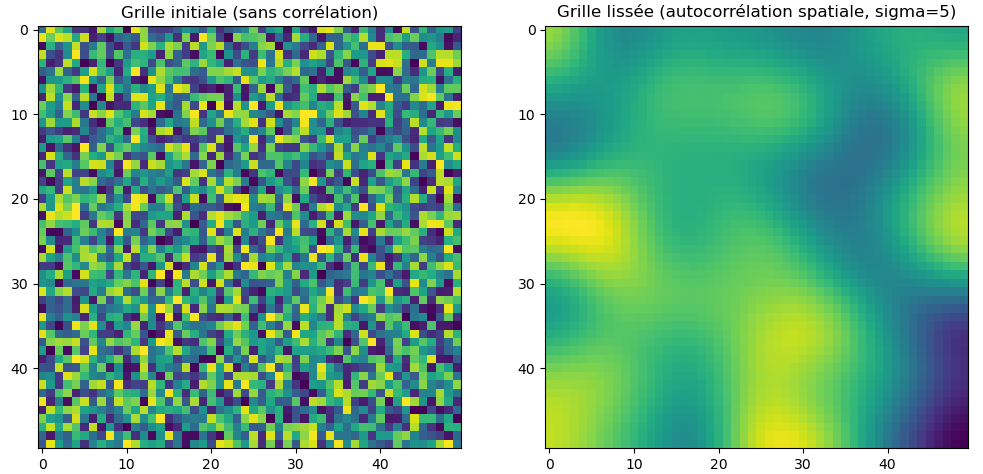
\includegraphics[width=0.95\textwidth]{images/autocorrelation.png}
    \caption{Illustration d'application de l'autocorrélation spaciale}
    \label{fig:autocorrelation}
\end{figure}
- Géostatistique : C'est une méthode d'analyse statistique utilisée pour modéliser et prédire des phénomènes spatiaux. Dans le cadre de l'interpolation, la géostatistique prend en compte l'autocorrélation spatiale des données pour effectuer des prédictions plus précises dans des régions non mesurées, en utilisant des techniques comme le krigeage (expliquée à la fin de cette section g).
Le kriging (ou krigeage en français) est une méthode d'interpolation géostatistique qui génère une estimation statistique des variables spatiales en tenant compte de l'autocorrélation spatiale. Cette méthode est particulièrement efficace pour capturer les comportements non linéaires des variables dans un ensemble de données.

La formule de base pour le kriging est :

\begin{equation}
    Z(x) = \sum_{i=1}^{N} \lambda_i \cdot Z(x_i)
\end{equation}

où :

- \( Z(x) \) : est la valeur interpolée au point \( x \).

\vspace{-0,2 cm}

- \( \lambda_i \) : sont les poids associés aux points de données \( x_i \), calculés en fonction de la covariance spatiale.

\vspace{-0,2 cm}

- \( Z(x_i) \) : est la valeur mesurée au point \( x_i \).

Le kriging permet non seulement de prédire les valeurs inconnues, mais aussi d'estimer l'incertitude associée à ces prédictions, ce qui en fait un outil puissant pour l'interpolation dans des domaines où les relations spatiales sont complexes.




\subparagraph{h.Cokriging \cite{kringing}}
\textit{Type : Géostatistique} \\
\phantom{----}Le cokriging est une extension multivariée du kriging, qui prend en compte la corrélation spatiale entre plusieurs variables. Il permet de modéliser simultanément plusieurs variables en utilisant des informations supplémentaires sur leurs corrélations spatiales. Cela peut améliorer la précision de l'interpolation dans les cas où plusieurs variables sont disponibles et corrélées.
%La formule pour le cokriging est similaire à celle du kriging, mais elle inclut des termes pour chaque variable considérée, ainsi que leurs covariances croisées. C'est l'extension multivariée du kringing.
%Cette méthode est particulièrement utilisée pour les applications où les variables ont des relations spatiales complexes et non linéaires, comme dans les simulations CFD (Computational Fluid Dynamics).
Voici une illustration du résultat de différentes méthodes d'interpolation venant du même article :
%"La pondération par l’inverse de la distance et les fonctions de base radiale sont des interpolateurs exacts, tandis que le polynôme global, le polynôme local, l’interpolation par noyaux avec interruptions et l’interpolation par diffusion avec interruptions sont inexacts."\footnote{https://pro.arcgis.com/fr/pro-app/latest/help/analysis/geostatistical-analyst/deterministic-methods-for-spatial-interpolation.html}
%Voici une classification des différentes méthodes d'interpolation géostatiques :
\begin{comment}
    \begin{figure}[H]
        \centering
        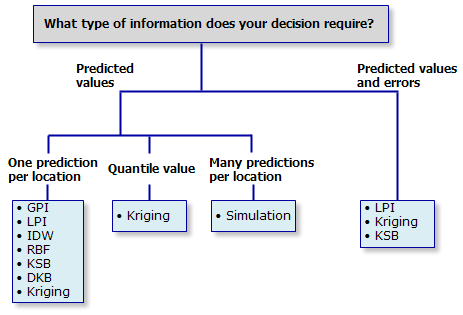
\includegraphics[width=0.75\textwidth]{images/arcgis.png}
        \caption{Arbre des méthodes d'interpolation géostatique (source : \href{https://pro.arcgis.com/fr/pro-app/latest/help/analysis/geostatistical-analyst/classification-trees-of-the-interpolation-methods-offered-in-geostatistical-analyst.htm}{pro.arcgis.com})}
    \label{fig:arcgis}
    \end{figure}
\end{comment}
%\subparagraph{a. Kriging et Cokriging} % traduction en Français : krigeage et cokrigeage
%Le kriging (ou krigeage en français) est une méthode d'interpolation géostatistique qui génère une estimation statistique des variables spatiales. Le cokriging est son extension multivariée. 

%La méthode kringing pourrait être un excellent candidat. Voici une traduction d'un extrait d'article discutant autour des résultats de cette méthode :
%"La méthode linéaire est simple, robuste et constitue un choix d'interpolation acceptable pour les premières estimations approximatives ou si les variables de la solution de la base de données dépendent linéairement des variables de l'espace de conception. La méthode IDW ne présente aucun avantage par rapport à la méthode linéaire plus simple et n'est pas recommandée pour l'interpolation des solutions CFD. La méthode de Krigeage donne les résultats interpolés les plus précis et permet de saisir le comportement non linéaire des variables de la solution de la base de données. Pour le cas d'essai AS-202, la différence maximale en pourcentage entre le taux de chauffage interpolé par la méthode de Krigeage et le taux de réchauffement CFD exact est inférieure à l'incertitude du taux de réchauffement CFD lui-même." \cite{palmer2009}

%ù"Le cokriging est l'extension multivariée du formalisme de Kriging, qui permet de traiter simultanément deux variables ou plus définies sur le même domaine et de prendre en compte des informations supplémentaires sur la corrélation spatiale entre les variables." \cite{kringing}

\begin{figure}[H]
    \centering
    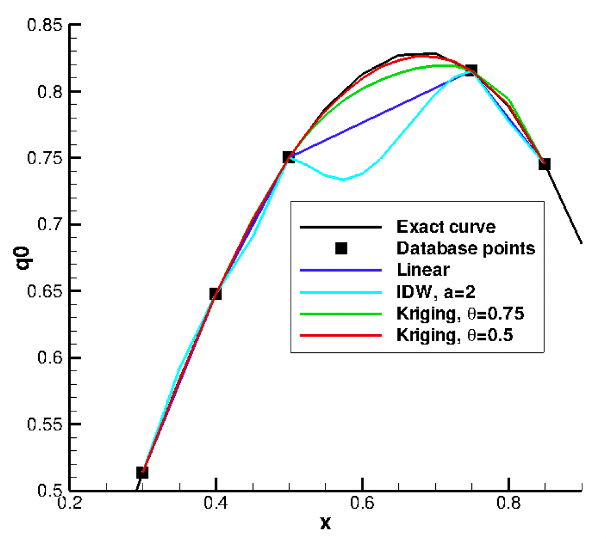
\includegraphics[width=0.55\textwidth]{images/palmer2009_comp_copie.png}
    \caption{Comparaison de différentes méthodes d'interpolation sur des données 1D (source \cite{palmer2009})}
    \label{fig:compar}
\end{figure}

\begin{comment}
    \subparagraph{b. DSM}
    La méthode \ac{DSM} pourrait s'avérer intéressante, car elle donne de meilleurs résultats que la méthode IDW dans le cas ...
     \cite{kim2019}
\end{comment}


%\subparagraph{b. IDW}
%Comme décrit plus tôt dans la partie 2.2.2, la méthode IDW se base sur la distance des points pour le calcul de l'interpolation. Elle est une application de la pondération de Shepard qui est elle-même une généralisation de l'approximation de Lagrange (à N-dimension).

\newpage

\subparagraph{i. RBF \cite{opencfs}}
\textit{Type : Base radiale} \\
\phantom{----}La \ac{RBF} est une fonction basée sur les distances telle que la méthode IDW. Cependant, elle peut utiliser différents types de bases radiales pour estimer la solution, telle que la base gaussienne, multiquadratique, etc. C'est un bon candidat pour une amélioration de l'interpolation IDW. Il faudrait ensuite trouver le meilleur noyau avec les meilleurs paramètres pour les cas d'applications rencontrés dans Antares. Pour des cas spécifiques tels que l'aéroacoustique, un petit algorithme itératif ou à base d'ajustement par la méthode des moindres carrés (voir méthode suivante) peut être mis en place pour trouver ces paramètres. Tel que l'interpolation linéaire, cette méthode n'est pas conservative (donc induis de la diffusion).
Voici la formule de la RBF pour un noyau \(\phi\) gaussien :
\begin{equation}
f(\mathbf{x}) = \sum_{i=1}^{N} w_{i} \, \varphi \left( \|\mathbf{x} - \mathbf{x}_{i}\| \right), \varphi(r) = e^{-(\epsilon r)^{2}}
\end{equation}

%Cette interpolation est utilisée et expliquée par un docteur en maths \cite{Rosenfeld}.%sur sa chaîne YouTube\footnote{http://www.thatmaththing.com/} et son site internet\footnote{http://www.thelearningdock.org/}.
Pour la prochaine méthode à implémenter : Des codes open source d'interpolation d'ordre élevé sont disponibles sur GitHub (en Julia \cite{opensource} et Python \cite{opensource_2} pour RBF et Noyaux de produits de points exponentiels) et expliqués par un docteur en maths \cite{Rosenfeld}. Les noyaux RBF gaussiens et les noyaux de produit de points exponentiels sont utilisés dans certaines interpolations. \cite{opensource_2}. La RBF est utilisée au CERFACS et disponible sur cloud2cloud.

\subparagraph{j. Les moindres carrés} %\label{mc}
\textit{Type : Outil} \\ %\vspace{0.2cm}
\phantom{----}
Cet outil vise à minimiser l'erreur quadratique pour créer une approximation des données. Elle est appliquée sur une fonction d'approximation paramétrable.

Des variantes plus performantes sont décrites dans le guide utilisateur de "hip".
Un logiciel créé en 1997 au CERFACS, nommé "hip" permet de convertir des maillages multi-blocs structurés en maillages non structurés.
Différentes méthodes d'interpolation y sont codées et décrites dans le guide utilisateur \cite{muller2020}.
Les approches d'interpolation linéaire par morceaux et par norme minimale sont plus rapides que la méthode des moindres carrés linéaires. \cite{muller2020}
%\subparagraph{3. Approximation des moindres carrés}
%\phantom{-}
%\newline
Approfondir des recherches sur la méthode \ac{MLS} \cite{MLS, levin} pourrait être intéressant.

\subparagraph{k. MISCOG}

\phantom{----}

Plusieurs méthodes innovantes d'interpolation d'ordre élevé sont déjà implémentées dans d'autres codes du CERFACS tel que dans les \ac{MISCOG} et un article les détaille \cite{laborderie2018}. Elles servent généralement pour d'autres applications comme pour calculer un flux au travers d'une cellule \cite{alexis} à l'aide d'une intégration sur une surface. Mais certaines parties sont intéressantes pour notre cas.




\newpage



\subsection{La méthode linéaire}
%\textit{Type : Polynomiale} \\
%\phantom{----}
La méthode linéaire est simple, robuste et constitue un choix d'interpolation acceptable pour les premières estimations approximatives ou si les variables de la solution de la base de données dépendent linéairement des variables de l'espace de conception \cite{palmer2009}.
%La littérature \cite{fluidssengineer} s'accorde à dire que l'interpolation linéaire, est la plus basique après plus proche voisin et IDW. J'entends par basique simple à implémenter, demandant peu de ressources, robuste et moyennement précise pour de l'ordre élevé. C'est pour cela que le CERFACS voulait l'implémenter dans Antares. C'est aussi la plus utilisée par Airbus, Safran et d'autres industriels (via d'autres codes qu'Antares). Cela est donc aussi intéressant d'avoir une interpolation linéaire directement dans Antares.

% Remplacer target par cible et point interpolé par cible.

\paragraph{1D}
\vspace{-0.5cm}
\subparagraph{Linéaire}
En 1D, l'interpolation linéaire est simple \cite{fluidssengineer, palmer2009}: c'est la moyenne pondérée linéairement par la distance, des valeurs des deux points les plus proches.
Supposons que nous voulons interpoler une valeur d'un point \( p \) entre deux points \( a \) et \( b \) dans un espace 1D
et que nous représentons leurs valeurs dans une deuxième dimension \( y \).
Nous aurons alors pour formule :

\begin{equation}
y_p = \frac{|x_b - x_p|}{|x_b - x_a|} \cdot y_a + \frac{|x_a - x_p|}{|x_b - x_a|} \cdot y_b
\end{equation}

%\vspace*{0.1\baselineskip}\linebreak
où \( y_p \) représente la valeur interpolée à la position \( x_p \), et \((x_a, y_a)\) et \((x_b, y_b)\) sont les points de référence. J'ai écrit cette formule afin qu'elle soit symétrique par rapport aux points \( a \) et \( b \), pour qu'ils jouent le même rôle. Ainsi elle s'entendra plus intuitivement dans des dimensions supérieures.
\vspace{0.5cm}
%\vspace*{0.1\baselineskip}\linebreak

        \( \frac{|x_b - x_p|}{|x_b - x_a|} \) est le poids pour \( y_a \) basé sur la distance relative de \( x_p \) à \( x_b \).

        \( \frac{|x_p - x_a|}{|x_b - x_a|} \) est le poids pour \( y_b \) basé sur la distance relative de \( x_p \) à \( x_a \).\vspace{0.5cm}

Ces deux termes sont pondérés de manière à ce que leur somme soit toujours égale à 1, ce
qui garantit que l'interpolation est correcte et symétrique par rapport à \( a \) et \( b \).\vspace{0.5cm}

\vspace{-0.5cm}

\paragraph{2D}
\phantom{-}

En 2D, nous devons nous baser sur des surfaces, extraites de formes pour pouvoir effectuer cette pondération. En CFD, ces formes sont appelées cellules et leurs sommets nœuds. Dans notre cas, nous considérons que les variables du maillage sont contenues au niveau des nœuds. 
Il existe 3 principaux types de cellules en 2D : les triangles, les rectangles des maillages structurés (dans ce cas, la méthode est dite bilinéaire) et les quadrilatères (non croisés).
Nous trouvons de plus en plus de polygones à N arêtes dans les maillages. Mais par souci de simplicité, l'interpolation linéaire se limite aux trois principaux types de cellules, les polygones pouvant être décomposés en triangles. % https://team.inria.fr/titane/files/2019/12/barycentric.pdf et https://www.inf.usi.ch/hormann/papers/Hormann.2014.BI.pdf  décris l'interpolation barycentrique généralisée

\subparagraph{Triangle : Barycentrique}

Pour le triangle, la méthode pour trouver la valeur au point à interpoler \( p \) est celle dite du barycentre (barycentrique).
Elle est bien documentée.
Visuellement, il faut faire la somme des valeurs aux points pondérés par la surface opposée et pondérer le tout par la surface du triangle.

\begin{comment}
    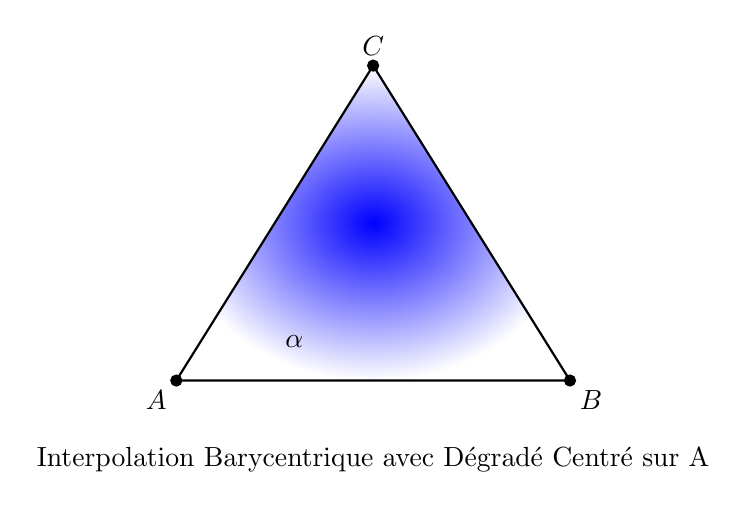
\begin{tikzpicture}
    % Triangle coordinates
    \coordinate (A) at (0,0);
    \coordinate (B) at (5,0);
    \coordinate (C) at (2.5,4);

    % Gradient fill centered at vertex A
    \shade[shading=radial, inner color=blue, outer color=white] (A) -- (B) -- (C) -- cycle;

    % Draw triangle
    \draw[thick] (A) -- (B) -- (C) -- cycle;

    % Draw labels and points
    \filldraw[black] (A) circle (2pt) node[anchor=north east] {$A$};
    \filldraw[black] (B) circle (2pt) node[anchor=north west] {$B$};
    \filldraw[black] (C) circle (2pt) node[anchor=south] {$C$};
    \node at (1.5,0.5) {$\alpha$};

    % Title
    \node at (2.5,-1) {Interpolation Barycentrique avec Dégradé Centré sur A};

\end{tikzpicture}
\end{comment}

\begin{figure}[H]
    \centering
    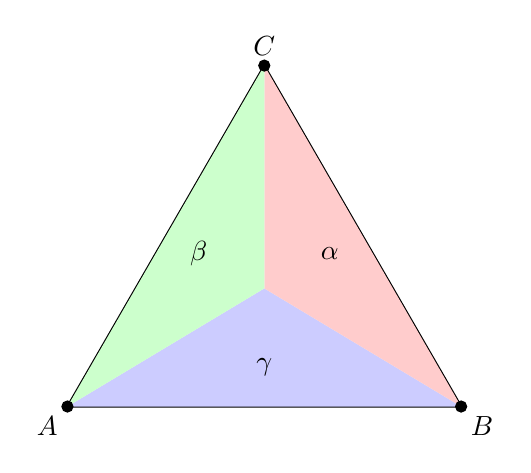
\begin{tikzpicture}

        % Define the triangle vertices
        \coordinate (A) at (0,0);
        \coordinate (B) at (5,0);
        \coordinate (C) at (2.5,4.33);
        \coordinate (P) at (2.5,1.5); % Point d'interpolation
    
        % Draw triangle
        \draw[thick] (A) -- (B) -- (C) -- cycle;
    
        % Draw Voronoi-like regions
        \fill[blue!20]  (A) -- (B) -- (P) -- cycle;
        \fill[red!20]   (B) -- (C) -- (P) -- cycle;
        \fill[green!20] (C) -- (A) -- (P) -- cycle;
        %\fill[green!20] (C) -- (barycentric cs:A=1,B=0,C=1) -- (barycentric cs:A=0,B=1,C=1) -- cycle;
    
        % Draw points
        \filldraw[black] (A) circle (2pt) node[anchor=north east] {$A$};
        \filldraw[black] (B) circle (2pt) node[anchor=north west] {$B$};
        \filldraw[black] (C) circle (2pt) node[anchor=south] {$C$};
    
        % Add labels
        \node at (barycentric cs:B=1,C=1,P=1) {$\alpha$};
        \node at (barycentric cs:C=1,A=1,P=1) {$\beta$};
        \node at (barycentric cs:A=1,B=1,P=1) {$\gamma$};
    
        % Title
        %\node at (2.5,-1) {Interpolation Barycentrique}; %Diagramme de Voronoi Modifié pour l'
    
    \end{tikzpicture}
    \label{fig:interpolation_barycentrique}
    \caption{Schéma d'interpolation barycentrique}
    %\label{fig:interpolation_IDW_rayon}
\end{figure}



Le calcul est le suivant :
\begin{equation}
    \frac{\alpha f(A) + \beta f(B) + \gamma f(C)}{\alpha + \beta + \gamma}
\end{equation}


\vspace{0.1cm}

Les triangles rencontrés sont quelconques, mais la formule reste la même.

% Trilinéaire dans le cas où le maillage est 3D et structuré.
\subparagraph{Rectangle : Bilinéaire}

En ce qui concerne l'interpolation bilinéaire sur un rectangle, nous la trouvons aussi facilement dans la littérature. La formule est l'extension de celle pour les triangles :

\vspace{-0.4cm}

\begin{equation}
    \resizebox{0.9\hsize}{!}{$
    f(x, y) = \frac{(x_2 - x)(y_2 - y)f_{11} + (x - x_1)(y_2 - y)f_{21} + (x_2 - x)(y - y_1)f_{12} + (x - x_1)(y - y_1)f_{22}}{(x_2 - x_1)(y_2 - y_1)}
    $}
\end{equation}
                
Nous supposons que le point cible est bien à l'intérieur du rectangle lorsque nous appliquons le calcul.
Dans la formule, les surfaces sont directement calculées dans \(f(x, y)\) contrairement à la méthode barycentrique où une étape de plus est nécessaire.
Cela correspond à l'addition de deux interpolations linéaires. Nous trouvons souvent dans la littérature une équation analytique où tous les sommets ne jouent pas le même rôle, mais il est plus simple de faire un calcul de poids pour pouvoir ensuite faire une moyenne pondérée. 
Visuellement, nous créons cette fois des traits parallèles en passant par le point d'interpolation et nous additionnons, de manière pondérée, les 4 surfaces multipliées chacune par leur sommet opposé respectif.

\begin{figure}[H]
    \centering
    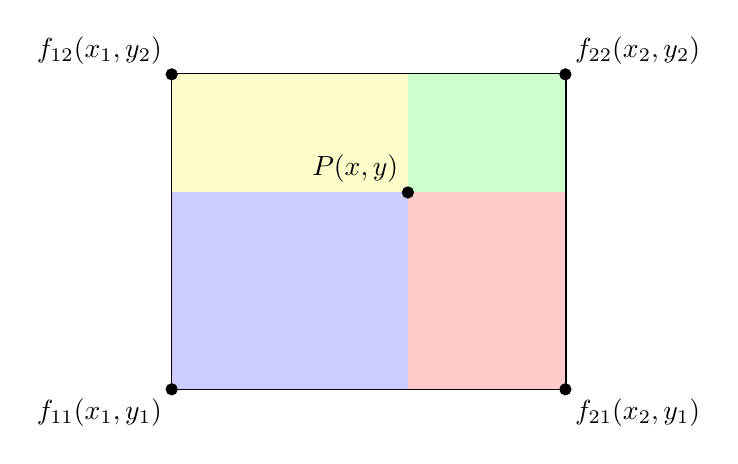
\begin{tikzpicture}
        % Define the rectangle vertices
        \coordinate (A) at (0,0);
        \coordinate (B) at (5,0);
        \coordinate (C) at (5,4);
        \coordinate (D) at (0,4);
        \coordinate (P) at (3,2.5); % Point d'interpolation
        
        % Draw rectangle
        \draw[thick] (A) -- (B) -- (C) -- (D) -- cycle;
        
        % Draw the perpendicular lines from P to the sides of the rectangle
        \draw[dashed] (P) -- (3,0);   % Vertical to the bottom side
        \draw[dashed] (P) -- (3,4);   % Vertical to the top side
        \draw[dashed] (P) -- (0,2.5); % Horizontal to the left side
        \draw[dashed] (P) -- (5,2.5); % Horizontal to the right side
        
        % Fill the areas
        \fill[blue!20]  (A) -- (3,0) -- (P) -- (0,2.5) -- cycle;
        \fill[red!20]   (B) -- (5,2.5) -- (P) -- (3,0) -- cycle;
        \fill[green!20] (C) -- (5,2.5) -- (P) -- (3,4) -- cycle;
        \fill[yellow!20] (D) -- (0,2.5) -- (P) -- (3,4) -- cycle;
        
        % Draw points
        \filldraw[black] (A) circle (2pt) node[anchor=north east] {$f_{11} (x_1, y_1)$};
        \filldraw[black] (B) circle (2pt) node[anchor=north west] {$f_{21} (x_2, y_1)$};
        \filldraw[black] (C) circle (2pt) node[anchor=south west] {$f_{22} (x_2, y_2)$};
        \filldraw[black] (D) circle (2pt) node[anchor=south east] {$f_{12} (x_1, y_2)$};
        \filldraw[black] (P) circle (2pt) node[anchor=south east] {$P (x, y)$};
        
        % Title
        %\node at (2.5,-1) {Interpolation Bilinéaire};
        %Interpolation Bilinéaire
    \end{tikzpicture}
    \caption{Schéma d'interpolation bilinéaire}
    %\label{fig:interpolation_IDW_rayon}
\end{figure}


\begin{comment}
    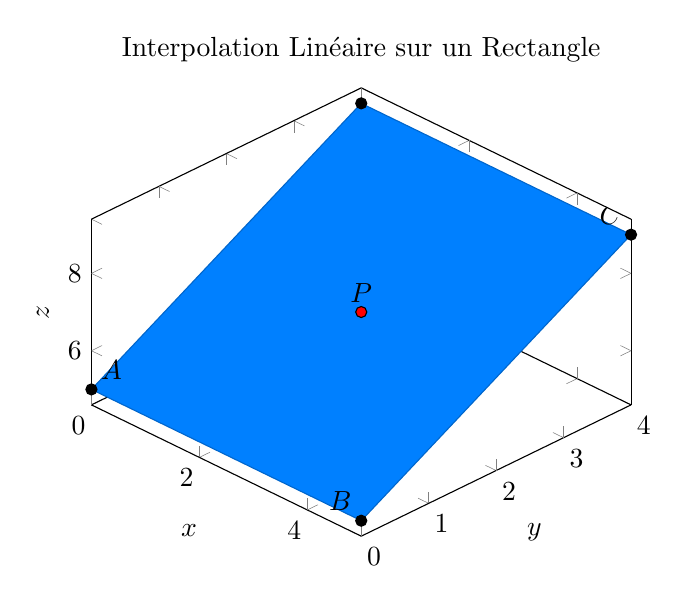
\begin{tikzpicture}
    \begin{axis}[
        view={45}{45},
        xlabel={$x$},
        ylabel={$y$},
        zlabel={$z$},
        colormap/cool,
        title={Interpolation Linéaire sur un Rectangle},
        ]

        % Define the vertices of the rectangle
        \addplot3[surf, mesh/rows=2, domain=0:5, domain y=0:4] 
            coordinates {(0,0,5) (5,0,5) (0,4,9) (5,4,9)};

        % Draw points for vertices and their labels
        \addplot3[only marks, mark=*] coordinates {(0,0,5) (5,0,5) (5,4,9) (0,4,9)};
        \addplot3[only marks, mark=*, mark options={fill=red}] coordinates {(2.5,2,7)};

        % Labels for the vertices and interpolated point
        \node at (axis cs:0,0,5) [anchor=south west] {$A$};
        \node at (axis cs:5,0,5) [anchor=south east] {$B$};
        \node at (axis cs:5,4,9) [anchor=south east] {$C$};
        \node at (axis cs:0,4,9) [anchor=south west] {$D$};
        \node at (axis cs:2.5,2,7) [anchor=south] {$P$};

    \end{axis}
    \end{tikzpicture}
\end{comment}

\newpage

\subparagraph{Quadrilatère}

Regardons maintenant le dernier type de cellule 2D rencontré dans les solutions traitées par Antares : les quadrilatères.
Pour cela, je n'ai pas trouvé de méthode satisfaisante dans la littérature \cite{perronnet1998}. Après plusieurs essais sur papier, je me suis concentré sur le fait que la méthode devait être continue, ce qui implique notamment que la valeur du point à interpoler doit tendre vers la valeur d'un sommet lorsque sa distance à ce dernier tend vers 0 et la linéarité doit être respecté entre deux points, sur les arêtes.
Une première contrôle de la linéarité est de vérifier qu'un point au milieu d'une cellule 2D a comme valeur la moyenne de ses sommets.
Via cette démarche, j'ai imaginé, graphiquement, tracer des traits entre le point à interpoler et les sommets de la cellule dans laquelle il se situe (tel que pour l'interpolation Barycentrique).
Cela permet de ne créer que quatre sous-formes.
Ensuite pour déterminer le poids associé au sommet \( s_1 \), il faut multiplier entre elles les deux surfaces qui lui sont opposées, et bien entendu, le pondérer une fois les autres poids calculés.
Par opposées, j'entends que ces surfaces ne sont composées d'aucunes arêtes ayant pour l'une de leurs extrémités le point d'interpolation. Ceci est important pour l'extension de l'idée en 3D.

\begin{figure}[H]
    \centering
    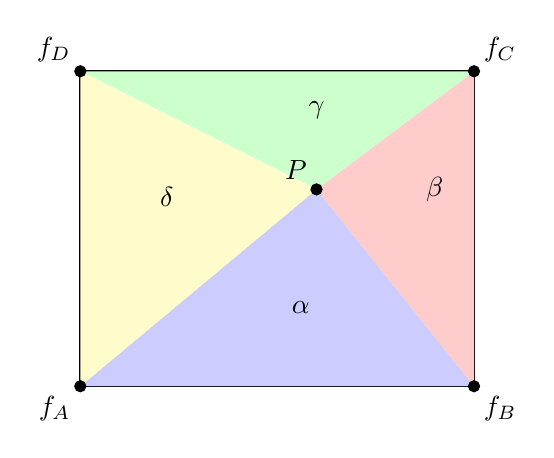
\begin{tikzpicture}
        % Define the rectangle vertices
        \coordinate (A) at (0,0);
        \coordinate (B) at (5,0);
        \coordinate (C) at (5,4);
        \coordinate (D) at (0,4);
        \coordinate (P) at (3,2.5); % Point d'interpolation
    
        % Draw rectangle
        \draw[thick] (A) -- (B) -- (C) -- (D) -- cycle;
    
        % Draw the interpolation lines parallel to the sides
        \draw[dashed] (P) -- (0,2.5); % Horizontal to the left side
        \draw[dashed] (P) -- (3,0);   % Vertical to the bottom side
        \draw[dashed] (P) -- (5,2.5); % Horizontal to the right side
        \draw[dashed] (P) -- (3,4);   % Vertical to the top side
    
        % Fill the areas
        \fill[blue!20]  (A) -- (P) -- (B) -- cycle;
        \fill[red!20]   (B) -- (P) -- (C) -- cycle;
        \fill[green!20] (C) -- (P) -- (D) -- cycle;
        \fill[yellow!20] (D) -- (P) -- (A) -- cycle;
    
        % Draw points
        \filldraw[black] (A) circle (2pt) node[anchor=north east] {$f_A$};
        \filldraw[black] (B) circle (2pt) node[anchor=north west] {$f_B$};
        \filldraw[black] (C) circle (2pt) node[anchor=south west] {$f_C$};
        \filldraw[black] (D) circle (2pt) node[anchor=south east] {$f_D$};
        \filldraw[black] (P) circle (2pt) node[anchor=south east] {$P$};
    
        % Add labels for the distances
        \node at (2.8, 1.0) {$\alpha$};%{$x_2 - x$};
        \node at (4.5, 2.5) {$\beta$};%{$y_2 - y$};
        \node at (3.0, 3.5) {$\gamma$};%{$x - x_1$};
        \node at (1.1, 2.4) {$\delta$};%{$y - y_1$};
    
        % Title
        %\node at (2.5,-1) {Interpolation dans un quadrilatère quelconque};
    
    \end{tikzpicture}
    \caption{Schéma d'interpolation dans un quadrilatère quelconque}
    \label{fig:quad}
    %\label{fig:interpolation_IDW_rayon}
\end{figure}

Un point à souligner est qu'une multiplication de surfaces est réalisée, qui induit une équation d'ordre 4, ce qui pourrait impliquer une méthode du même ordre.
Contrairement à son nom, l'interpolation bilinéaire est en réalité quadratique avec un résultat linéaire.
Une vérification a été faite et la méthode interpole avec de l'erreurs les fonctions d'ordre supérieur à un.
De plus, le quadratique ne peut pas englober le linéaire dans le cas où nous nous basons uniquement sur les quatre points d'un quadrilatère.
% Effectivement, en 1D, si nous avons \(f(x_i)\) = 0 et \(f(x_{i+1})\) = 1, le résultat d'une variable linéaire serait 0,5 et celui d'une variable quadratique 0,25, si nous avons uniquement connaissance de ces deux points.
Normalement il faudrait s'appuyer sur plus de points pour le quadratique. 
Finalement, la démonstration pourrait se construire en montrant la linéarité selon les axes x et y indépendamment (comme pour le bilinéaire). En effet, sur la Figure \ref{fig:quad} ci-dessus, nous remarquons que lors d'un déplacement selon l'horizontal, vers la droite, les surfaces \(\alpha\) et \(\gamma\) ne varient pas tandis que la surface \(\delta\) augment linéairement et \(\beta\) diminue linéairement aussi.
Voici l'équation de la méthode d'interpolation linéaire pour le quadrilatère :

\begin{equation}
    f(P) = \frac{f_{A} \cdot (\beta \times \gamma) + f_{B} \cdot (\gamma \times \delta) + f_{C} \cdot (\delta \times \alpha) + f_{D} \cdot (\alpha \times \beta)}{(\beta \times \gamma) + (\gamma \times \delta) + (\delta \times \alpha) + (\alpha \times \beta)}
\end{equation}
    

\vspace{0.2cm}  % OU \\[0pt plus 1fill] OU \newline OU flushleft, flushright, center


\paragraph{3D}
\subparagraph{Pavé droit : Trilinéaire}

Pour le 3D, si le maillage est structuré, alors le type de cellule est le pavé droit. À ce moment, nous sommes dans le cas de l'interpolation dite trilinéaire. La formule se trouve facilement dans la littérature et peut être retrouvée par extension de la formule de l'interpolation sur un rectangle. Nous associons comme poids à un des huit sommets \( s_1 \) le volume opposé, construit tel que sur la Figure \ref{fig:trilineaire}

\begin{figure}[H]
    \centering
    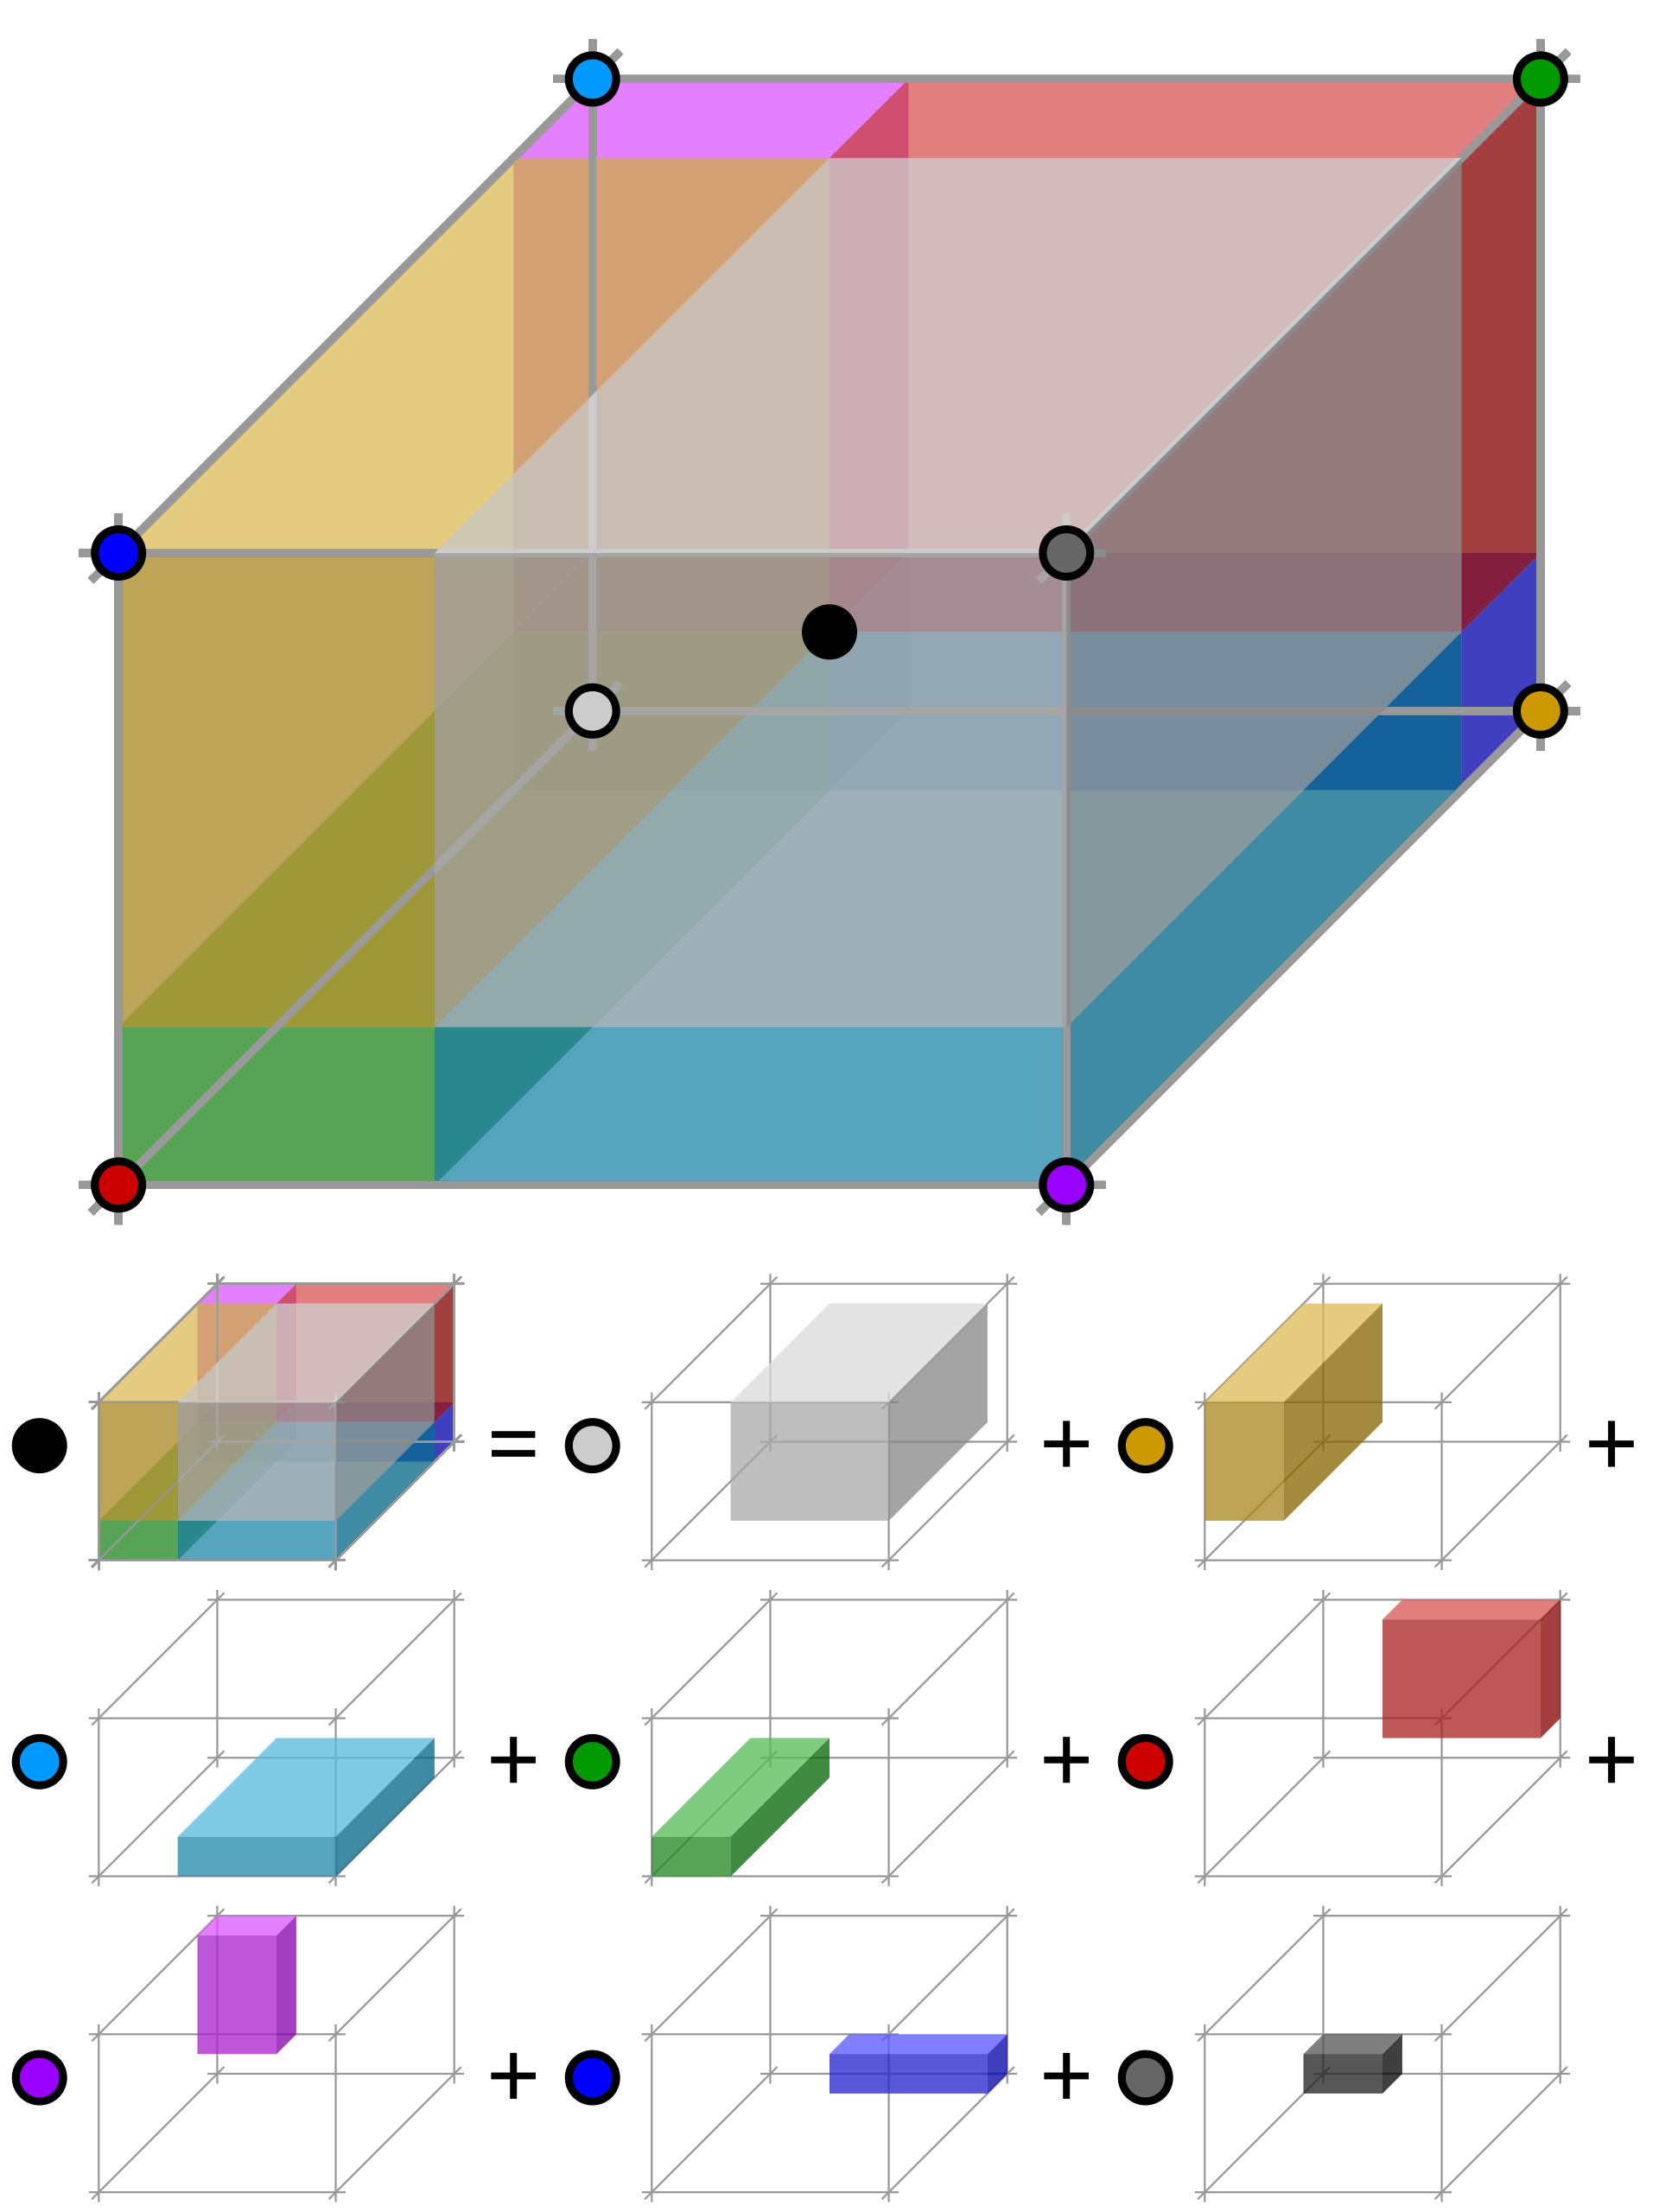
\includegraphics[width=0.4\textwidth]{images/Trilinear_interpolation_visualisation.svg.png}
    \caption{Schéma d'interpolation trilinéaire (source : Wikipédia)} %\footnote{Source:https://en.wikipedia.org/wiki/Trilinear_interpolation#/media/File:Trilinear_interpolation_visualisation.svg}}
    %\label{fig:https://en.wikipedia.org/wiki/Trilinear_interpolation#/media/File:Trilinear_interpolation_visualisation.svg}
    \label{fig:trilineaire}
\end{figure}

L'équation qui en découle est la suivante :

\begin{equation}
    f(x, y, z) = \sum_{i=0}^{1} \sum_{j=0}^{1} \sum_{k=0}^{1} f_{ijk} (1 - |x - x_i|)(1 - |y - y_j|)(1 - |z - z_k|)
\end{equation}

% Expliquer mathématiquement ? Ou plus tard dans le code ?  (quadrilatère non croisé, concave et convexes)

% En CFD il y a toujours des formes, même si c'est structuré, on peut unstructure.

\subparagraph{Tétraèdre : Barycentrique étendu}

Pour le tétraèdre (une pyramide à base triangulaire quelconque), nous trouvons bien un volume opposé à chaque sommet. Opposé dans le sens où le sommet ne partage pas de segment avec le volume. Nous pouvons alors appliquer la même formule que pour le triangle, avec 4 volumes à la place de 3 surfaces.

\subparagraph{Pyramide, hexaèdre, prisme et autres formes}

Pour la pyramide (à base quadrilatérale) et l’hexaèdre, une extension de la formule du quadrilatère sera faite.
Il pourrait en être de même pour les prismes et autres formes, mais des problèmes d'implémentation apparaissent (partie \ref{prisme}).


Note pour l'ordre supérieur : une transformation des quadrilatères vers des rectangles pourrait être faite afin de pouvoir appliquer les équations d'interpolation \cite{camarero2024}. Cela peut être étendu au 3D.


%\subsection{Résumé des similitudes et différences des différentes méthodes}


\newpage
\section{Implémentation de la méthode linéaire}

\subsection{La structure générale du code "TreatmentInterpolation"}

Après avoir recensé les différentes méthodes qui seraient applicables, ma seconde mission a été d'implémenter une interpolation linéaire dans Antares. Grâce à Nitrox, j'ai accès au code source de la librairie que je peux modifier. Le code 'interpolation.py' est orienté objet et fait environ mille lignes. 
Il prend comme arguments obligatoires (Tableau \ref{tab:arguments_interpolation1}) la base source et la base cible et renvoie dans le cas le plus simple la base cible avec les valeurs interpolées.
De manière simplifiée, dans le code, les zones de la base source sont fusionnées puis les instants sont parcourus. 
Cette fusion permet de faire un \ac{KDTree}, qui permet concrètement de rechercher de manière efficace quels sont les \( N \) points de la base source les plus proches des points de la base cible (et les distances associées, utilisées dans la méthode 'idw').
Cette structure de données arborescente est conçue pour organiser des points dans un espace à k dimensions, ce qui est particulièrement utile pour effectuer des recherches rapides de voisins dans un ensemble de données multidimensionnelles.
Le KDTree divise récursivement l'espace en sous-espaces plus petits en utilisant des plans perpendiculaires aux axes de coordonnées. À chaque niveau de l'arbre, les points sont séparés en fonction de l'une des dimensions, avec une alternance de dimensions à chaque niveau. Cette approche hiérarchique permet de partitionner l'espace de manière efficace, rendant la recherche des points voisins beaucoup plus rapide que si l'on comparait chaque point individuellement.
Ensuite l'interpolation est calculée par l'une des deux méthodes 'principales' qui peut elle-même appeler d'autres fonctions ou méthodes d'Antares.
Voici les arguments initialement présents dans le code d'interpolation :


\label{arguments}
\begin{table}[ht]
    \centering
    \begin{tabular}{|l|l|l|}
    \hline
    \textbf{Nom} & \textbf{Val. défaut} & \textbf{Description} \\ \hline %    \textbf{Nom} & \textbf{\shortstack{Valeur\\par défaut}} & \textbf{Description} \\ \hline
    %\multicolumn{3}{|l|}{\textbf{Arguments présent initialement}} \\ \hline
    \texttt{source} & \texttt{N/A} & Base source \\
    \texttt{target} & \texttt{N/A} & Base cible \\
    \texttt{coordinates} & \texttt{None} & Le nom des variables de coordonnées spatiales \\
    \texttt{variables} & \texttt{None} & Nom des variables à interpoler (toutes pas défaut) \\
    \texttt{tolerance} & \texttt{1e-10} & Seuil de proximité pour utiliser la valeur du point \\
    \texttt{\phantom{-}} & \texttt{\phantom{-}} &  le plus proche \\
    \texttt{duplicated\_tolerance} & \texttt{None} & Nbr de décimales d'arrondi pour la détection de \\
    \texttt{\phantom{-}} & \texttt{\phantom{-}} & points dupliqués (exact par défaut) \\
    \texttt{invdist\_power} & \texttt{1} & Paramètre de puissance \(p\) de la méthode IDW \\
    \texttt{nb\_points} & \texttt{None} & Paramètre de nombre de points \(N\) de la méthode IDW \\
    \texttt{with\_boundaries} & \texttt{False} & Utiliser ou non les données des limites \\ \hline
    %\multicolumn{3}{|l|}{\textbf{Arguments ajoutés}} \\ \hline
    %\texttt{tolerance\_edge} & \texttt{1e-10} & Tolerance 'point dans la cellule ?' (ref \ref{pt_cell})\\
    %\texttt{method} & \texttt{'idw'} & Méthode d'interpolation ('idw' ou 'linear') \\
    %\texttt{data} & \texttt{None} & Mettre les données pré-calculées \\
    %\texttt{get\_data} & \texttt{None} & True pour récupérer des données \\ \hline
    \end{tabular}
    \caption{Arguments initiaux pour la méthode d'interpolation dans Antares}
    \label{tab:arguments_interpolation1}
\end{table}

%Tolérance relative entre la somme des sous-surfaces créées par le point p et la surface totale de la cellule pour déterminer si un point est dans une cellule ou non\label{pt_cell}

\begin{comment}
    LIST_KEYS = [{'name': 'source'},
    {'name': 'target'},
    {'name': 'coordinates',
     'default': None},
    {'name': 'variables',
     'default': None},
    {'name': 'tolerance',
     'default': 1e-10},
    {'name': 'duplicated_tolerance',
     'default': None},
    {'name': 'invdist_power',
     'default': 1},
    {'name': 'nb_points',
     'default': None},
    {'name': 'with_boundaries',
     'default': False}]
+
    {'name': 'tolerance_edge',
     'default': 1e-10},
    {'name': 'method',
     'default': 'idw'},
    {'name': 'data',
     'default': None},
    {'name': 'get_data',
     'default': None}
\end{comment}





\label{implementation_IDW}\paragraph{L'interpolation IDW}

%Cette distance est définie à 1e-10 dans le traitement et peut être modifiée par l'utilisateur en ajustant l'argument \texttt{'tolerance'} en ajoutant la ligne
La méthode IDW contient deux paramètres \(N\) et \(p\) (section \ref{sIDW})
Par défaut, dans le code, \(p\) est égal à '1' et \(N\) est égale au nombre de sommets de la première cellule de la liste de types de cellules de la base cible. Il y aurait peut-être une modification mineure à faire sur ce point. La structure de la base cible importe peu comparée à celle de la base source, pour l'interpolation. Mais par souci de rétrocompatibilité, aucune modification ne doit changer l'utilisation qui a déjà été faite de ce traitement. % ! test à faire ici !
Ces paramètres peuvent être changés par l'utilisateur ajoutant
\begin{lstlisting}[]
    myt['tolerance'] = valeur
\end{lstlisting}
entre la ligne 2 et 5 de l'exemple présenté dans la partie '2.1 La librairie Antares' avec pour respectivement \texttt{'nb\_points'} et \texttt{'invdist\_power'}.\label{parametres}

Une de mes missions était de chercher s'il y avait des paramètres plus optimisés que \(N\) et \(p\) pour cette méthode. Je n'ai pas trouvé la réponse dans les différents articles \cite{idw-arcgis} et thèses que j'ai lues. C'est pour cela qu'il sera présenté plus tard dans le rapport comment des paramètres optimaux ont été trouvés en faisant des tests.

\label{prisme}\paragraph{L'interpolation linéaire}

%"La méthode linéaire est simple, robuste et constitue un choix d'interpolation acceptable pour les premières estimations approximatives ou si les variables de la solution de la base de données dépendent linéairement des variables de l'espace de conception" \cite{palmer2009}.
La littérature \cite{fluidssengineer, palmer2009} s'accorde à dire que l'interpolation linéaire est plus précise et robuste que la méthode du plus proche voisin et IDW, peu coûteuse et simple à implémenter. C'est pour cela que le CERFACS voulait l'implémenter dans Antares. C'est la plus utilisée par Airbus, Safran et d'autres industriels (via d'autres codes qu'Antares). Il est donc intéressant d'avoir une interpolation linéaire directement dans Antares.

Le traitement d'interpolation linéaire d'Antares ne traite que des maillages ayant des valeurs uniquement au niveau des nœuds des cellules (pas dans les cellules ou entre les nœuds). Cela est dû à la manière dont est structurée notre méthode d'interpolation linéaire. % (\lstinline{__idw_interpolate_instant} ou \lstinline{__barycentrique_interpolate_instant})
La méthode ne fonctionne pas pour tous les cas de connectivité prismatique, notamment pour les cellules constituées de triangles non parallèles entre elles dans l'espace et de surfaces différentes. De plus, l'ordre des sommets contenu dans la connectivité est différent en fonction du solveur dont est issue la base (par exemple dans hip elle est définie tel que sur l'image \annexref{fig:ordre_connect}). Telle que la méthode a été implémentée, cela rend le calcul des volumes presque impossible. Nous avons effectivement besoin de savoir à quel sommet correspond quel indice. La connectivité prismatique ne sera donc finalement par traitée. Il en est de même pour les cellules plus complexes à N faces ou toute autre connectivité qui viendrait à apparaître.
Cependant, ce problème peut être pallié. Il faut "tétraèdriser" la base source afin de créer des tétraèdres avant d'utiliser le traitement d'interpolation. Il en est de même pour de potentiels cas 2D non traités.
Voici comment réaliser cela :

\begin{lstlisting}[caption=Utilisation du traiement "tetrahedralize" pour interpoler linéairement tous types de cellules, label={lst:tet}]
    import antares
    from copy import deepcopy
    # deepcopy est utilise pour ne pas "tetrahedralize" la 'source_base' 
    
    copy_source_base = deepcopy(source_base)
    # copy_source_base.unstructure() # Pour une base non structure
    t = antares.Treatment('tetrahedralize')
    t['base'] = copy_source_base
    copy_source_base = t.execute()

    myt = antares.Treatment('interpolation')
    myt['source'] = copy_source_base
    myt['target'] = target_base
    result2 = myt.execute()
\end{lstlisting}

Lorsque la base est structurée, il n'y a pas de connectivité facilement accessible, donc pas d'interpolation linéaire implémentée. Il faut donc '\texttt{unstructure}' la base source puis la "tétraèdriser". Cela s'effectue de la même façon que définie dans le code ci-dessus, en ajoutant 
\begin{lstlisting}[]
    copy_source_base.unstructure()
\end{lstlisting}
à la ligne 6 du code \ref{lst:tet}. Dans les faits, le traitement sur maillage structuré a été développé pour l'ordre un et deux, avec un bug pour l'ordre trois. Par manque de temps, l'implémentation de la méthode n'a pas été finalisée. Étant généralement plus rapide que l'interpolation IDW, la fonctionnalité sera possiblement disponible plus tard.


\newpage
\subsection{Le pseudo-algorithme}

Voici le pseudo-algorithme simplifié donnant l'architecture de la fonction linéaire du traitement interpolation. Elle est appliquée à toutes les zones qui sont fusionnées et un seul instant à la fois.

\vspace{0.3cm}

\textbf{Initialisation :}

$\bullet$ Créer le KD-tree

$\bullet$ Créer une liste de listes \texttt{node\_to\_elements} qui permet de récupérer l'indice des éléments constitués par un certain point.

$\bullet$ Définir les points à interpoler

\vspace{0.5cm}

\textbf{Parcours des points à interpoler :}
\begin{list}{$\circ$}{\leftmargin=0.5cm \labelwidth=1cm \itemsep=0cm}
    \item Pour chaque point :
    \begin{list}{$\diamond$}{\leftmargin=0.5cm \labelwidth=1cm \itemsep=0cm}
        \item Si la distance au point le plus proche est inférieure à \texttt{tolerance} :
        \begin{list}{$\bullet$}{\leftmargin=0.5cm\labelwidth=1cm \itemsep=0cm}
            \item Le poids associé au \texttt{point cible} prend la valeur 1
            \item Le sommet associé au \texttt{point cible} prend la valeur du \texttt{point source} le plus proche
        \end{list}
        \item Sinon :
        \begin{list}{$\bullet$}{\leftmargin=0.5cm \labelwidth=1cm \itemsep=0cm}
            \item Récupérer les indices des éléments des points les plus proches\\
            $\circ$ Pour chaque élément pertinent :
            \begin{list}{$\bullet$}{\leftmargin=0.5cm\labelwidth=1cm \itemsep=0cm}
                \item Récupérer les coordonnées des sommets (points) de la cellule\\
                $\diamond$ Si le point est à l'intérieur de la cellule :
                \begin{list}{$\bullet$}{\leftmargin=0.5cm \labelwidth=1cm \itemsep=0cm}
                    \item Calculer les poids 'barycentriques'
                    \item Récupérer les indices des sommets (points) de la base source
                \end{list}
            \end{list}
        \end{list}
    \end{list}
    $\diamond$ Si le point n'est dans aucune cellule proche :
    \begin{list}{$\bullet$}{\leftmargin=0.5cm \labelwidth=1cm \itemsep=0cm}
        \item Le poids associé prend la valeur \texttt{numpy.nan} (cette valeur sera changée avant la mise à jour d'octobre)
    \end{list}
\end{list}

\vspace{0.4cm}

\begin{comment}
    Premièrement, dans \lstinline{__barycentrique_interpolate_instant}, nous récupérons le nombre de points maximal sur lequel nous allons nous appuyer pour l'interpolation, soit le nombre maximal de sommet des cellules présentes dans le maillage.
    Nous récupérons les distances et indices du KDTree.
    Ensuite nous devons réarranger des indices qui se sont fait déplacer lors de la fusion des zones.
    Nous récupérons aussi différentes variables, comme les coordonnées des points, \dots
\end{comment}

%Nous récupérons d'une fonction définie plus bas (\lstinline{get_list_cell_type}) :
%(\lstinline{list_cell_type, max_node_index})

%\noindent Dans le cas où le maillage est le même entre tous les instants, ou que l'utilisateur a déjà récupéré les poids (et autres valeurs utiles) nous ne recalculons pas tous les paramètres, ce qui permet une diminution significative du temps de calcul.

\textbf{Mise à jour de la base cible :}
\begin{list}{$\circ$}{\leftmargin=0.5cm \labelwidth=1cm \itemsep=0cm}
    \item Pour chaque variable à interpoler :
    \begin{list}{$\bullet$}{\leftmargin=0.5cm \labelwidth=1cm \itemsep=0cm}
        \item La variable de chaque nouveau point prend la valeur des poids calculés multipliés par la variable aux sommets (points) respectifs de la base source
    \end{list}
\end{list}


%Expliquer 'is point on cell', etc...

%% \subsection{Les difficultés}

\subsection{Optimisation du temps de calcul}

Plusieurs axes ont été exploités afin de diminuer le temps de calcul du traitement d'interpolation.

Le premier est de ne calculer qu'une seule fois le couple (poids, indices des points source) et les autres paramètres puis de les enregistrer. Cela est utile dans deux cas : %Le premier a été énoncé dans le pseudo-algorithme présenté dans la section précédente. Il s'agit

- Entre les instants si la structure des deux bases reste inchangée.
C'est par exemple dans le cas des bases issues de solutions aéroacoustiques. Dans le cas test d'aéroacoustique présenté section \ref{s241}, la solution contient deux cents instants, avec la méthode linéaire, le temps de calcul est divisé par plus de cent. Dans le code, un test est réalisé pour savoir si tous les instants sont partagés (section 2.1). Si oui, alors les poids et autres données nécessaires sont calculés. Ensuite, tous les instants seront calculés avec ces données.
Cette optimisation est faite automatiquement dans le traitement.
%\label{instants_partages}  % (grace à la variable \texttt{computation})  % , mais pas le premier instant.

- Si le calcul sur la base source est réalisé plusieurs fois sans que sa structure soit changée, qu'elle ait un instant ou plusieurs instants partagés. Dans le cas où la structure du maillage est différente entre deux instants, si l'argument \texttt{get\_data} a la valeur \texttt{True}, alors le programme renverra une erreur.
Un cas où l'on pourrait imaginer utiliser cette fonctionnalité est lors de plusieurs simulations avec des résultats physiques différents entre les simulations, mais toujours sur le même maillage. Pour utiliser cette fonctionnalité, il faut légèrement changer l'appel à la fonction, voici un exemple :

\begin{lstlisting}[caption=Exemple de réutilisation des données, label={lst:antares}]
    import antares
    from copy import deepcopy
    # deepcopy est utilise pour s'assurer que la 'target_base' ne soit pas calculee par le traitement

    myt = antares.Treatment('interpolation')
    myt['source'] = source_base
    myt['target'] = deepcopy(target_base)
    myt['get_data'] = True
    result1, data = myt.execute()

    # 'data' peut etre enregistre sur votre ordinateur par exemple, pour pouvoir etre appele plus tard

    myt = antares.Treatment('interpolation')
    myt['source'] = source_base
    myt['target'] = target_base
    myt['data'] = data
    result2 = myt.execute()
\end{lstlisting}

Ici, \texttt{result2} aura été calculé beaucoup plus rapidement que \texttt{result1}. De plus, ce changement est aussi appliqué à la méthode IDW sans poser de problèmes de rétrocompatibilité, car les résultats sont inchangés. Pour le cas test d'aéroacoustique à deux cents instants partagés, le traitement est cinq fois plus rapide pour l'IDW et plus de cent fois plus rapide pour la méthode linéaire.


La méthode linéaire était initialement deux cents à cinq cents fois plus lente que IDW. En faisant du 'profiling' pour savoir quelles lignes de code étaient les plus coûteuses, la rapidité a pu être augmentée. Certaines listes ont été remplacées par des tableaux NumPy avec une taille préallouée, ce qui améliore la rapidité d'insertion de nouvelles valeurs.

Le test de localisation d'un point dans une cellule et de calcul des poids a aussi été optimisé : les surfaces créées par le point cible avec les sommets sont calculées ainsi que le volume total de la cellule. Si la somme des sous-surfaces et égale à la surface totale de la cellule à une erreur numérique près, alors le point est dans la cellule et les poids sont déjà calculés. Sinon, il faut nécessairement chercher ailleurs. Un point à noter est que si le point est sur une arête, il pourrait ne jamais être détecté. Alors un argument \texttt{tolerance\_edge} a été créé. Si la tolérance relative entre la somme des sous-surfaces créées par le point p et la surface totale de la cellule est inférieure à \texttt{tolerance\_edge}, alors le point est considéré comme dans la cellule. %\label{pt_cell}

Ce test de localisation est coûteux, il a donc mené à autre idée de méthode qui a été testée pour réduire le temps de calcul. Elle reste linéaire, mais ne donne pas nécessairement le même résultat (lorsque la variable à interpoler est non-linaire, sinon le résultat reste la solution analytique). Cette idée est décrite uniquement pour le cas 2D par souci de simplicité de visualisation, mais est similaire pour le 3D.
Le principe est de ne pas calculer tout ce qui est en lien avec la connectivité, car c'est ce qui augmente significativement le temps de calcul.
Nous allons alors chercher les 3 (4 en 3D) points les plus proches. En reliant les sommets, cela donnera une forme (dite non croisée). 
Ensuite, nous faisons le calcul des barycentres et appliquons la même méthode que celle présenté dans le paragraphe précédent. Cela permet aussi une extrapolation linéaire sans créer d'erreur.
La différence avec la méthode classique est que le point cible n'est pas nécessairement dans la cellule décrite par les 3 points les plus proches.


\begin{figure}[H]
    \centering
    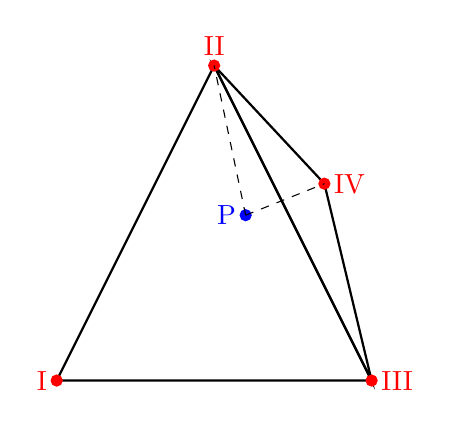
\begin{tikzpicture}
        \centering
        % Triangle initial
        \coordinate (I) at (0,0);
        \coordinate (II) at (2,4);
        \coordinate (III) at (4,0);
        \coordinate (P) at (2.4,2.1); % Point P (plus proche du nouveau triangle)

        % Nouveau triangle
        \coordinate (IV) at (3.4,2.5);

        % Draw the initial triangle
        \draw[thick] (I) -- (II) -- (III) -- cycle;

        % Draw the new triangle
        \draw[thick] (II) -- (III) -- (IV) -- cycle;

        % Draw point P
        \filldraw[blue] (P) circle (2pt) node[anchor=east] {P};

        % Label the vertices of the initial triangle
        \filldraw[red] (I) circle (2pt) node[anchor=east] {I}; % [anchor=east,xshift=-5pt,yshift=-5pt]
        \filldraw[red] (II) circle (2pt) node[anchor=south] {II};
        \filldraw[red] (III) circle (2pt) node[anchor=west] {III};

        % Label the vertices of the new triangle
        \filldraw[red] (IV) circle (2pt) node[anchor=west] {IV};

        % Draw lines from P to vertices
        \draw[dashed] (P) -- (IV);
        \draw[dashed] (P) -- (II);

        % Title
        %\node at (4,-1) {P plus proche de IV que du sommet le plus éloigné du triangle dans lequel il se trouve};
    \end{tikzpicture}
    \caption{Schéma de sélection du deuxième point le plus proche}
    \label{fig:deux_pt}
%\label{fig:interpolation_IDW_rayon}
\end{figure}


Alors nous pourrions avoir une ou des surfaces formées par le point cible qui sortent du triangle initial (et la somme des surfaces ne serait pas égale à la surface du triangle initial). Mais pour respecter la linéarité, il suffit de faire le même calcul en prenant en compte le fait que la ou les deux surface(s) entièrement extérieures à la cellule sont négatives. La figure ci-dessous (Figure \ref{fig:surface_negative}) est un zoom sur la Figure \ref{fig:deux_pt}.

\begin{figure}[H]
    \centering
    \begin{tikzpicture}
        % Triangle initial
        \coordinate (II) at (2*1.5,4*1.5);
        \coordinate (III) at (4*1.5,0);
        \coordinate (P) at (2.4*1.5,2.1*1.5); % Point P (plus proche du nouveau triangle))
        \coordinate (IV) at (3.4*1.5,2.5*1.5);
    
        % Draw point P
        \filldraw[blue] (P) circle (2pt) node[anchor=east] {P};
    
        % Label the vertices of the initial triangle
        \filldraw[red] (II) circle (2pt) node[anchor=south] {II};
        \filldraw[red] (III) circle (2pt) node[anchor=west] {III};
    
        % Label the vertices of the new triangle
        \filldraw[red] (IV) circle (2pt) node[anchor=west] {IV};
    
        % Colorer les surfaces, avec une surface négative
        \fill[blue!20] (II) -- (P) -- (IV) -- cycle;
        \fill[green!20, opacity=1.0] (III) -- (P) -- (IV) -- cycle;
        % Utilisation de hachures pour indiquer une surface négative
        \fill[pattern=north west lines, pattern color=red, opacity=0.7] (P) -- (III) -- (II) -- cycle;
    
        % Draw the 'outside' triangle
        \draw[thick] (II) -- (III) -- (IV) -- cycle;
    
        % Draw lines from P to vertices
        \draw[thick] (P) -- (IV);
        \draw[thick] (P) -- (II);
        \draw[thick] (P) -- (III);
    
        % Ajouter des annotations pour indiquer la surface négative
        %\node at (2.1*1.5,2.15*1.5) [anchor=west] {Surface};
        %\node at (2.1*1.5,2.15*1.5-0.4) [anchor=west] {négative};
        \node at (3, 1) [anchor=east] {
            \begin{tikzpicture}[baseline]
                \fill[pattern=north west lines, pattern color=red, opacity=0.7] (0,0) rectangle (0.5,0.2);
            \end{tikzpicture}
            \hspace{0.1cm} Surface négative
        };
        %\node at (3, 1) [anchor=east] {Surface négative};
        \draw[->, thick] (3, 1) -- (4.0, 2.9);

        %\node at (2.5*1.5, 1.5*1.5) [anchor=north] {\textbf{-}};
    \end{tikzpicture}    
    \caption{Illustration de la surface négative avec le point P}
    \label{fig:surface_negative}
\end{figure}


N'ayant pas trouvé une façon simple de savoir si la surface était négative, par manque de temps et crainte de l'ajout de complexité (qui augmente possiblement le temps de calcul), cette méthode n'a pas été implémentée.

Finalement, voici les arguments ajoutés pour la méthode linéaire :

\label{arguments_ajoutes}
\begin{table}[H]
    \centering
    \begin{tabular}{|l|l|l|}
    \hline
    \textbf{Nom} & \textbf{Val. défaut} & \textbf{Description} \\ \hline %    \textbf{Nom} & \textbf{\shortstack{Valeur\\par défaut}} & \textbf{Description} \\ \hline

    %\multicolumn{3}{|l|}{\textbf{Arguments ajoutés}} \\ \hline
    \texttt{method} & \texttt{'idw'} & Méthode d'interpolation ('idw' ou 'linear') \\
    \texttt{tolerance\_edge} & \texttt{1e-10} & Tolerance de 'point dans la cellule ?' \\
    \texttt{get\_data} & \texttt{None} & True pour récupérer des données \\ 
    \texttt{data} & \texttt{None} & Assigner les données précalculées \\ \hline
    \end{tabular}
    \caption{Arguments ajoutés pour la méthode d'interpolation dans Antares}
    \label{tab:arguments_interpolation2}
\end{table}

\begin{comment}
    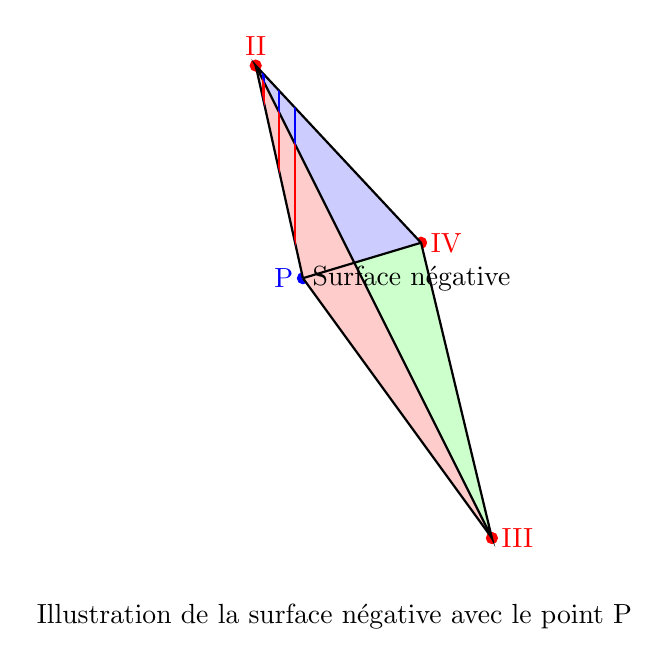
\begin{tikzpicture}
    \centering
    % Triangle initial
    \coordinate (II) at (2*1.5,4*1.5);
    \coordinate (III) at (4*1.5,0);
    \coordinate (P) at (2.4*1.5,2.2*1.5); % Point P (plus proche du nouveau triangle))
    \coordinate (IV) at (3.4*1.5,2.5*1.5);

    % Draw point P
    \filldraw[blue] (P) circle (2pt) node[anchor=east] {P};

    % Label the vertices of the initial triangle
    \filldraw[red] (II) circle (2pt) node[anchor=south] {II};
    \filldraw[red] (III) circle (2pt) node[anchor=west] {III};

    % Label the vertices of the new triangle
    \filldraw[red] (IV) circle (2pt) node[anchor=west] {IV};

    % Colorer les surfaces, avec une surface négative
    \fill[blue!20] (II) -- (P) -- (IV) -- cycle;
    \fill[green!20] (III) -- (P) -- (IV) -- cycle;
    \fill[red!20] (P) -- (III) -- (II) -- cycle; % Cette surface sera considérée comme négative

    % Draw the 'outside' triangle
    \draw[thick] (II) -- (III) -- (IV) -- cycle;

    % Draw lines from P to vertices
    \draw[thick] (P) -- (IV);
    \draw[thick] (P) -- (II);
    \draw[thick] (P) -- (III);

    % Hachures manuelles pour la surface bleue
    \begin{scope}
        \clip (II) -- (P) -- (IV) -- cycle;
        \foreach \x in {1.5,1.7,...,3.5} {
            \draw[blue, thick] (\x,-1) -- (\x,6);
        }
    \end{scope}

    % Hachures manuelles pour la surface verte
    \begin{scope}
        \clip (III) -- (P) -- (IV) -- cycle;
        \foreach \x in {1.5,1.7,...,3.5} {
            \draw[green, thick] (\x,-1) -- (\x,6);
        }
    \end{scope}

    % Hachures manuelles pour la surface rouge (négative)
    \begin{scope}
        \clip (P) -- (III) -- (II) -- cycle;
        \foreach \x in {1.5,1.7,...,3.5} {
            \draw[red, thick] (\x,-1) -- (\x,6);
        }
    \end{scope}

    % Ajouter des annotations pour indiquer la surface négative
    \node at (2.4*1.5,2.2*1.5) [anchor=west] {Surface négative};
    
    % Title
    \node at (4,-1) {Illustration de la surface négative avec le point P};
\end{tikzpicture}
\end{comment}

%\subsection{Le résultat}


\section{Tests}
A présent, le but est de savoir quelle est la méthode la plus précise, notamment dans le cas de l'interpolation pour l'application au traitement FWH. Pour cela il faut tester si la méthode linéaire fonctionne correctement, et tester les meilleurs paramètres \(N\) et \(p\) de la méthode IDW.%Tous les codes utilisés sont accessibles dans le répertoire \texttt{/archive/stg-cfds/thibault} sur kraken.
Améliorer la précision peut aussi permettre indirectement de réduite le coût de calcul. En déraffinant le maillage source, nous augmentons l'erreur, notamment dans le cadre de l'aéroacoustique \cite{schoder2019}, mais nous diminuons le temps de calcul. Ainsi, déraffiner le maillage source et utiliser une méthode d'interpolation précise peut permettre de réduire le temps de calcul tout en conservant la qualité des résultats finaux. %la perte de temps due à une méthode d'interpolation plus précise peut être compensée en déraffinant le maillage source.

\subsection{Tests unitaires sur la méthode linéaire}

Par manque de temps, il a été démontré uniquement par l'expérimentation que la méthode implémentée était linéaire.

Le premier test est de créer une variable linéaire et de faire une interpolation sur un second maillage. Ce test a été créé en même temps que l'implémentation dans l'objectif de tester si la méthode fonctionne dans un cas simple. Pour cela, on créé une base source avec une variable linéaire et une base cible avec des points décalés. Ensuite, on teste que l'interpolation renvoie bien la valeur analytique espérée sur tous les types de cellules. En comparant les valeurs analytiques et numériques, l'erreur observée est nulle. Ce test est effectué simplement avec une commande 'pytest' dans le terminal. Il est par ailleurs implémenté (pour la connectivité linéaire, triangulaire, quadrilatérale, tétraédrique et hexaédrique) dans les tests unitaires d'Antares, qui permettent de savoir que la librairie fonctionne correctement, notamment lors d'un git push vers Nitrox. Cependant, il est plus difficile de créer de manière simple un maillage avec des pyramides ou tétraèdres en python.
Une vue en coupe sur une base avec ces deux types de cellules a été utilisé pour compléter le test du code d'interpolation linéaire. La base contient une variable linéaire, et nous vérifions bien que l'erreur est nulle. Voici une visualisation (sur le logiciel Paraview) de l'interpolation linéaire Figure \ref{fig:lin_pyr_tet} (parfaitement lisse) que nous avons aussi comparé avec l'interpolation IDW Figure \ref{fig:idw_pyr_tet} qui s'avère moins "lisse".
\begin{figure}[H]
    \centering
    \begin{minipage}[t]{0.48\textwidth}
        \centering
        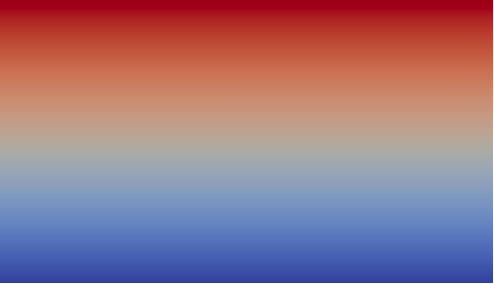
\includegraphics[width=\textwidth]{images/lin_pyr_tet2.png}
        \caption{Vue en coupe sur des cellules pyramidales et tétraédriques par interpolation linéaire}
        \label{fig:lin_pyr_tet}
    \end{minipage}%
    \hfill
    \begin{minipage}[t]{0.48\textwidth}
        \centering
        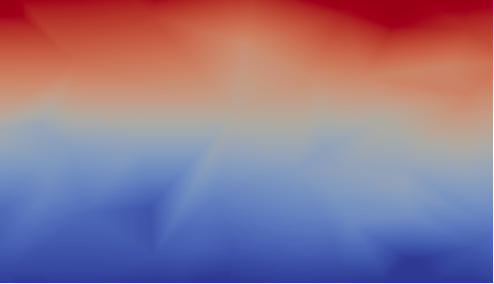
\includegraphics[width=\textwidth]{images/idw_pyr_tet2.png}
        \caption{Vue en coupe sur des cellules pyramidales et tétraédriques par interpolation idw}
        \label{fig:idw_pyr_tet}
    \end{minipage}
\end{figure}



Ensuite, j'ai essayé de tracer le log de l'erreur au sens des moindres carrés en fonction du raffinement du maillage source. Cela a étonnamment montré une convergence d'ordre quatre pour tous types de cellules (alors que nous nous attendions à une convergence d'ordre un pour le 1D). En voici l'exemple pour le 1D (Figure \ref{fig:bi}). Pour les autres types de cellules, les courbes sont similaires.
\begin{figure}[H]
    \centering
    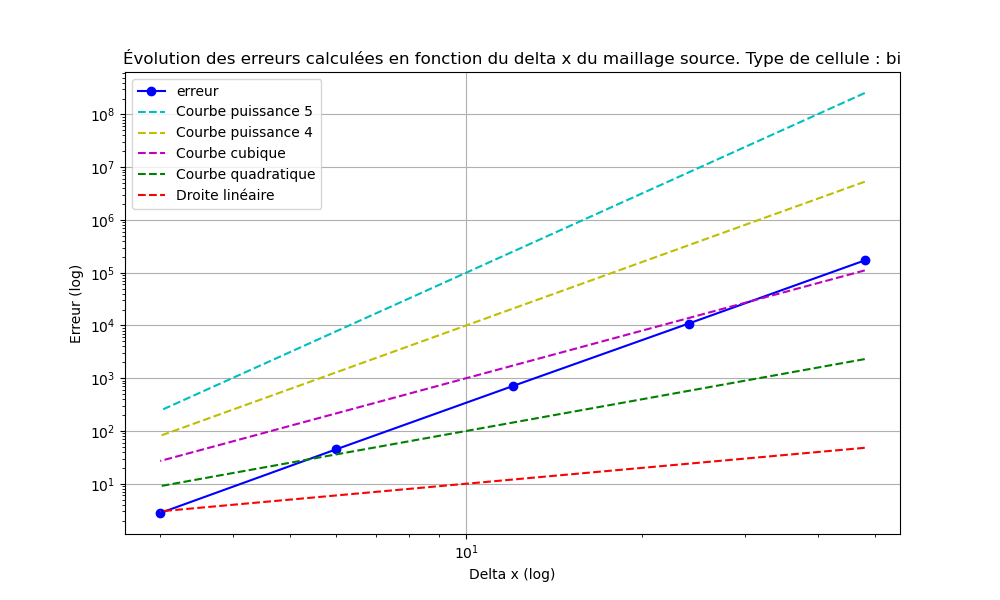
\includegraphics[width=0.90\textwidth]{images/err_puissance2_bi.png}
    \caption{Log de l'erreur en fonction du log du raffinement}
    \label{fig:bi}
\end{figure}


\subsection{Tests sur des cas industriels}

Pour tester la robustesse du traitement (notamment dans les cas multizones, multiconnectivités et multi-instants) il a été testé sur des cas industriels.
Voici deux images (Figure \ref{fig:cb-IDW} et Figure \ref{fig:cb-lineaire}) comparant l'interpolation IDW et linéaire sur un maillage 3D solution d'une flamme dans une chambre de combustion en base source et un plan en base cible qui coupe la base source en (0, 0, 0.01), selon l'axe z.

\begin{figure}[H]
    \centering
    \begin{minipage}[b]{0.47\textwidth}
        \centering
        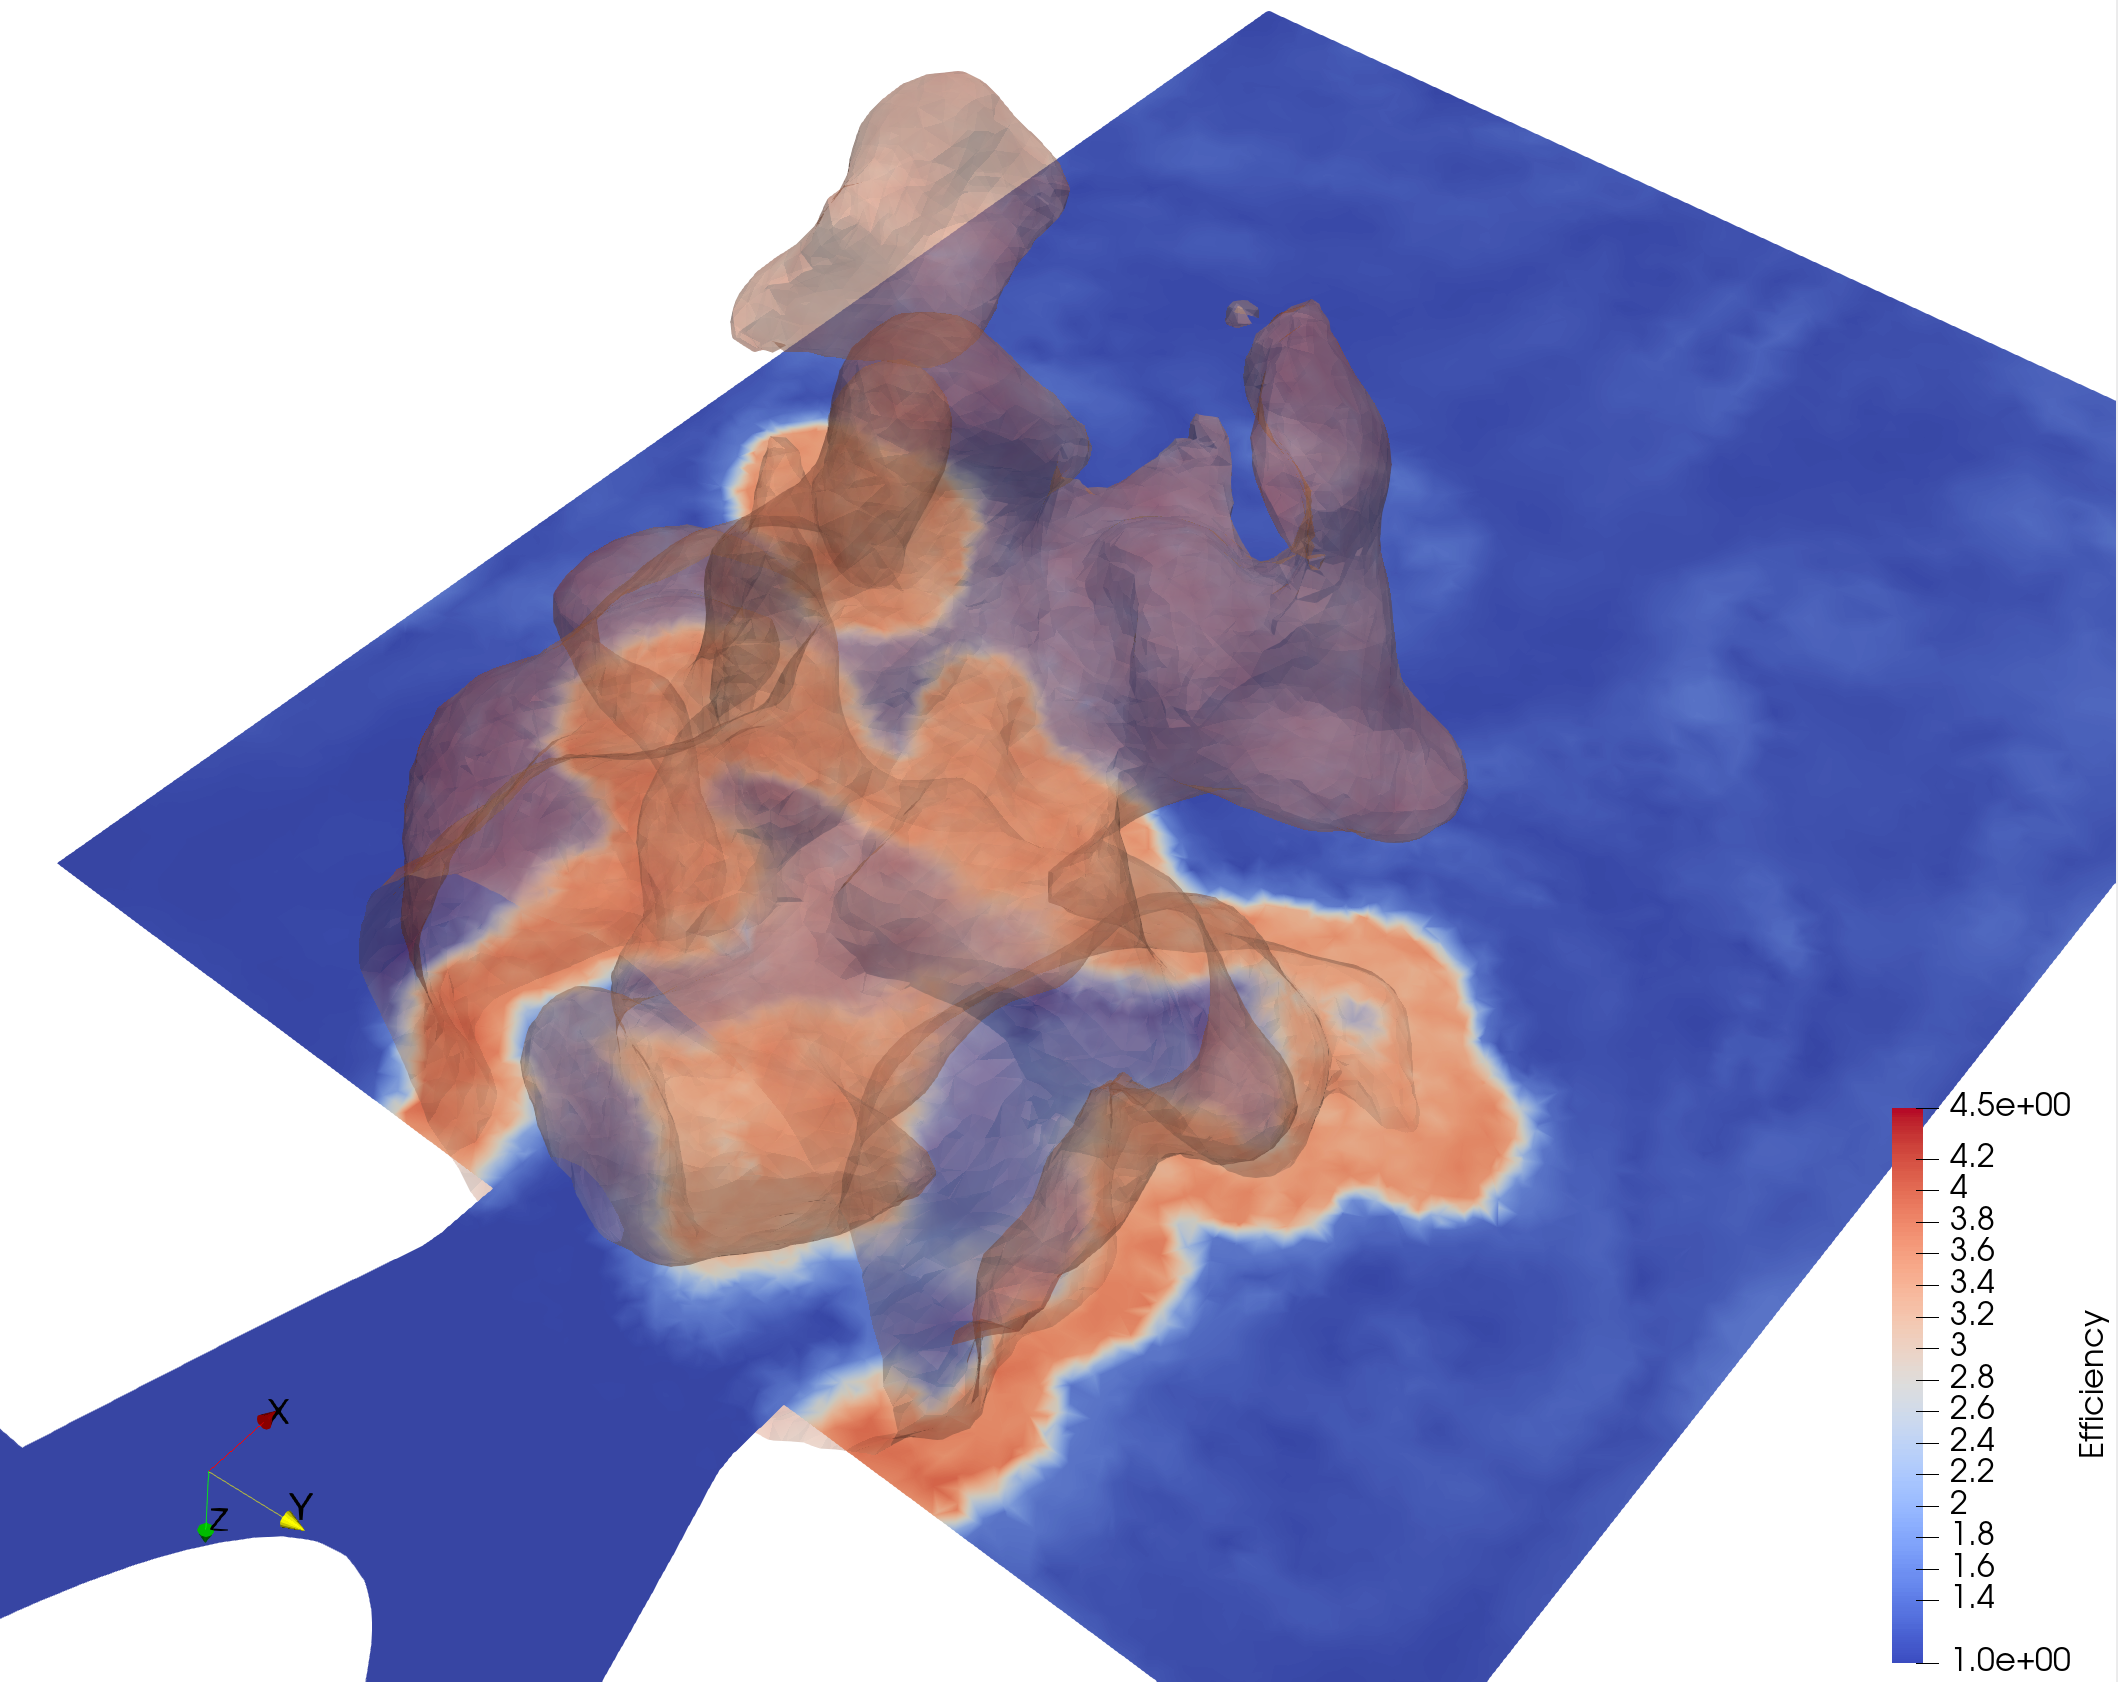
\includegraphics[width=\textwidth]{images/cb-IDW.png}
        \caption{Interpolation IDW sur une coupe d'une chambre de combustion avec isosurface de la flame}
        \label{fig:cb-IDW}
    \end{minipage}
    \hspace{0.02\textwidth} % Espace entre les deux figures
    \begin{minipage}[b]{0.47\textwidth}
        \centering
        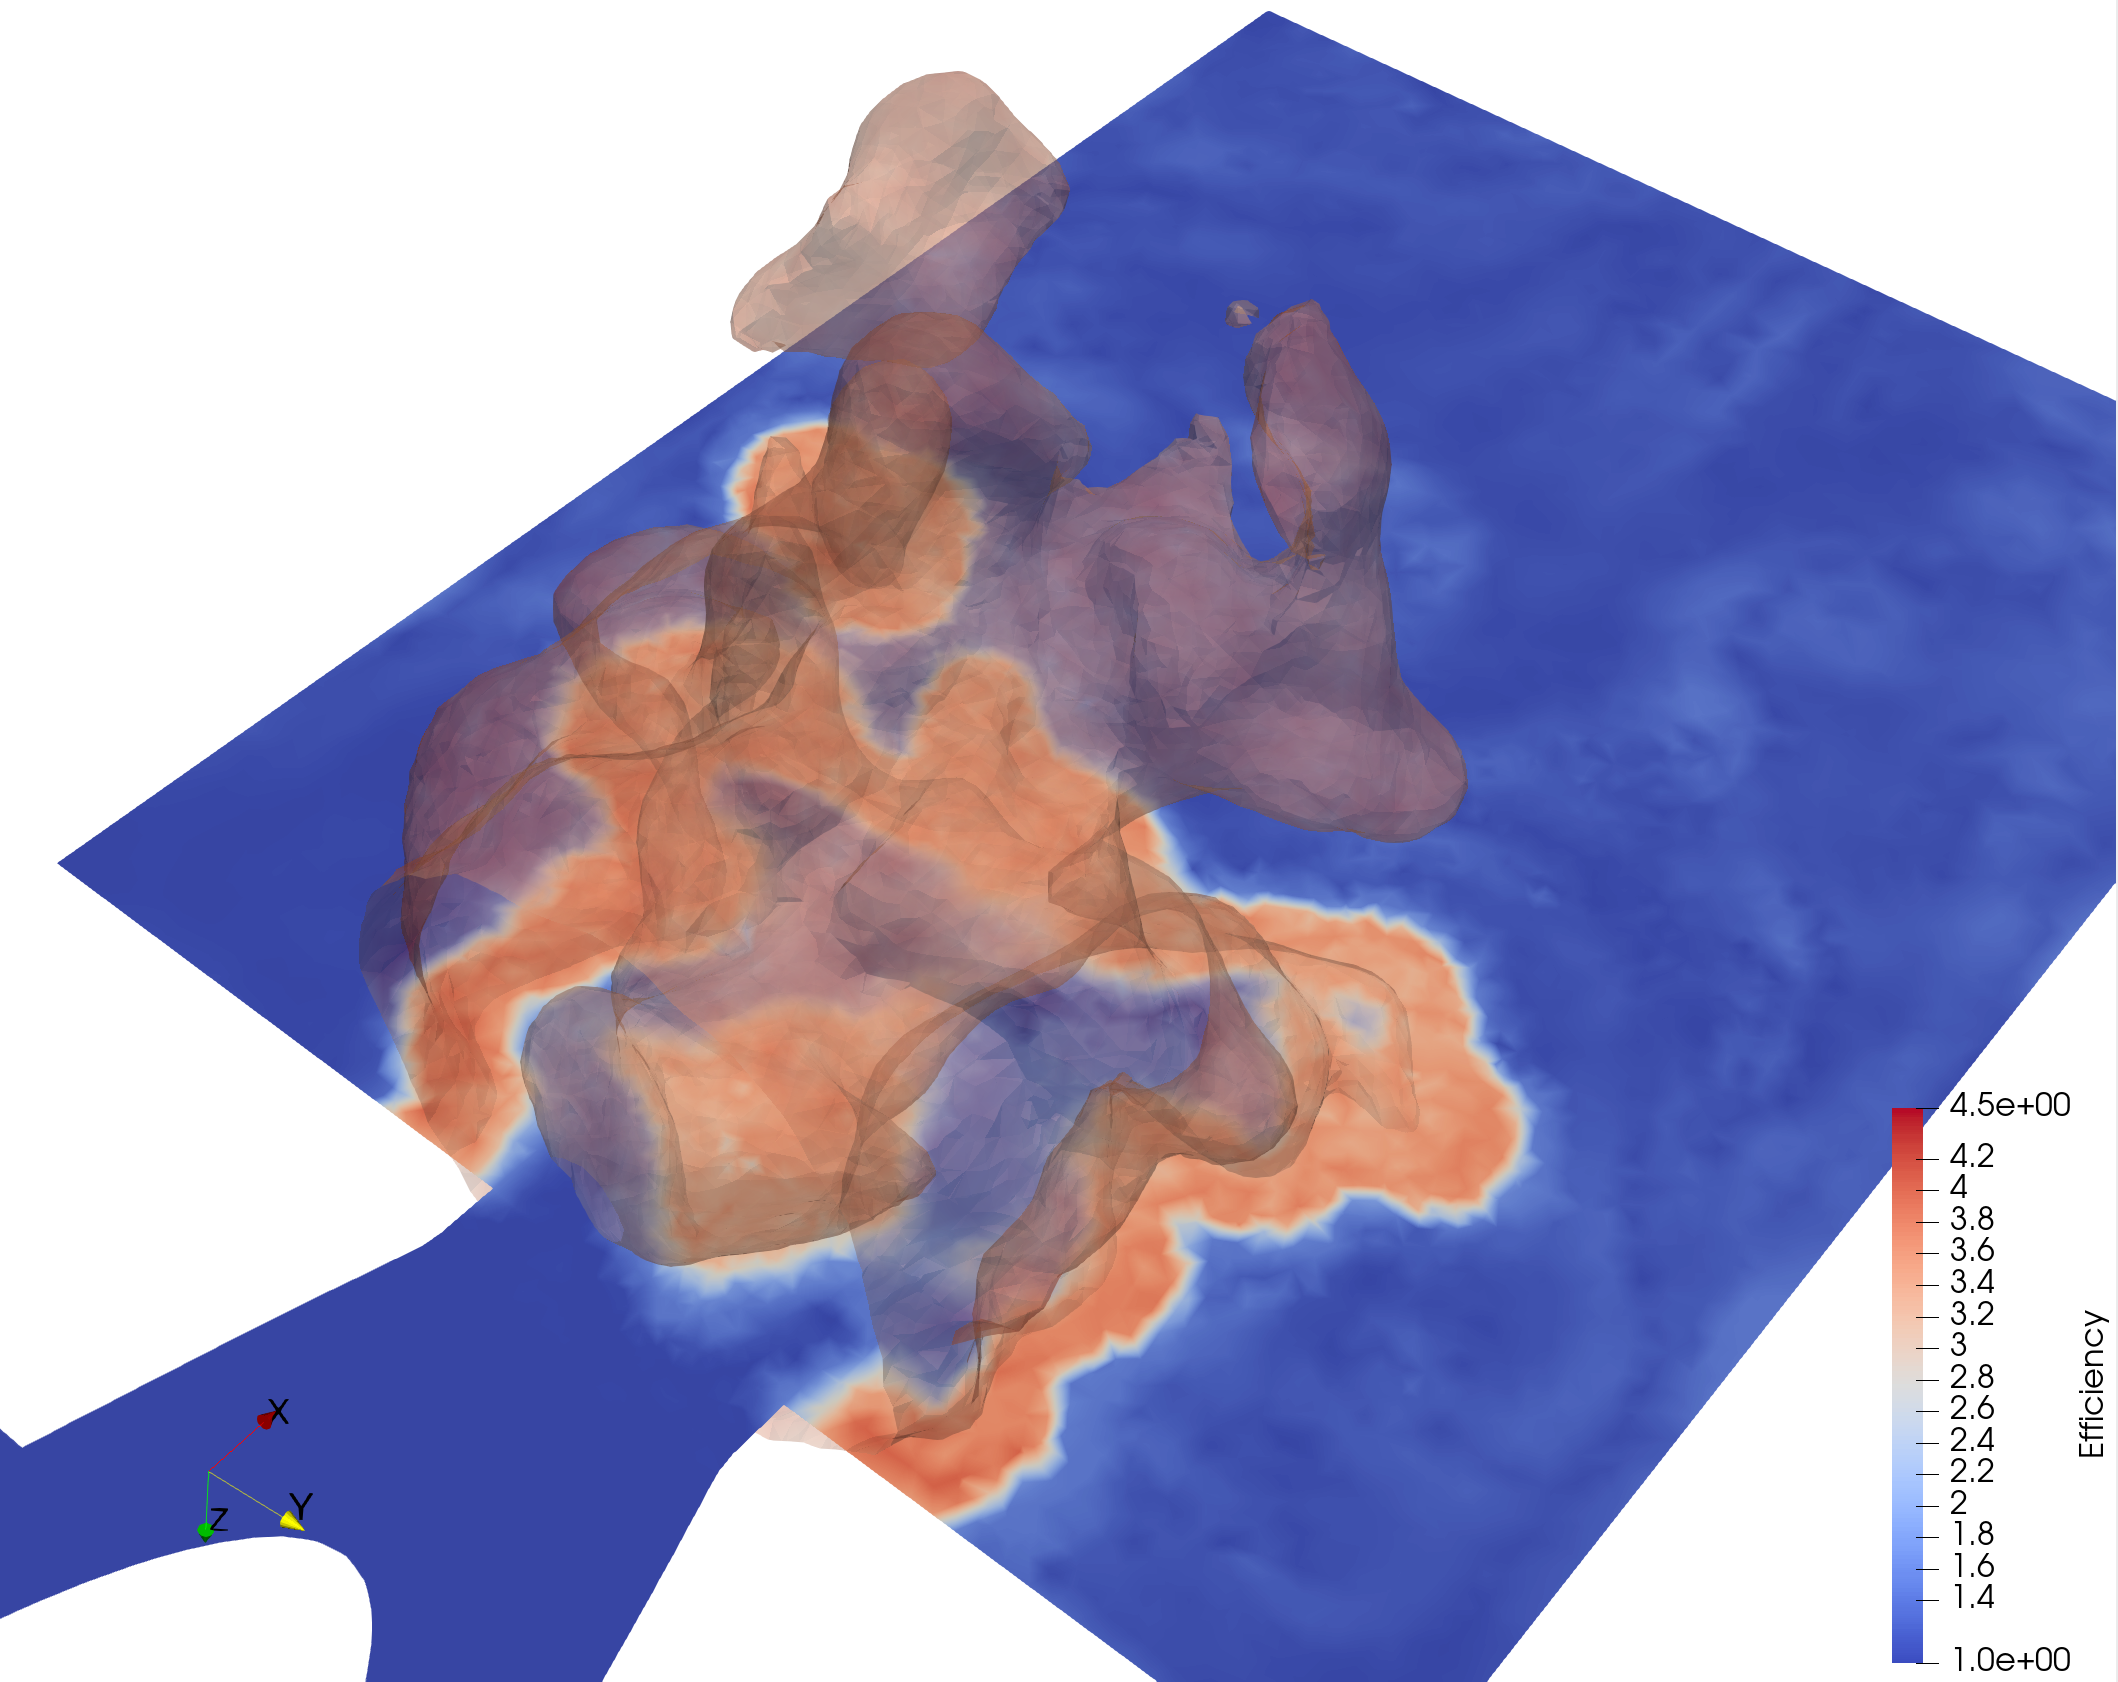
\includegraphics[width=\textwidth]{images/cb-lineaire.png}
        \caption{Interpolation linéaire sur une coupe d'une chambre de combustion avec isosurface de la flame}
        \label{fig:cb-lineaire}
    \end{minipage}
\end{figure}


Nous observons bien que les résultats sont similaires dans les deux cas (avec de légères différences démontrant que les méthodes sont bien différentes).

Voici les résultats de temps de calcul et d'erreur avec l'interpolation du logiciel vtk :

- Interpolation linéaire :         16.634 s, MSE: 1.7e-28

\vspace{-0,2cm}

- Interpolation IDW :\hspace{0,4cm} 0.661 s, MSE: 4.0e-03

\vspace{-0,2cm}

- Rapport de temps de calcul linéaire/IDW: 25

L'erreur au sens des moindres carrés est quasiment nulle pour l'interpolation linéaire, nous en déduisons que vtk interpole aussi linéairement. L'erreur numérique correspond probablement à une méthode d'interpolation linéaire différente utilisée par vtk mais le résultat théorique est le même.

\subsection{Tests sur des cas d'aéroacoustique}\label{s241}

Le traitement FWH permet de déterminer le son à grande distance émanant d'une source aéroacoustique. Cela peut être utilisé pour déterminer numériquement le bruit d'un moteur d'avion par exemple.
Dans notre cas test, la source n'est pas un moteur, mais une onde aéroacoustique simulée dans un cube.
Voilà comment fonctionne notre chaîne aéroacoustique.\label{s243}
Nous créons une base source rectangulaire, sur cette image (Figure \ref{fig:aac1}) elle est constituée de 3x5 nœuds et $4^3$ éléments.
Nous lui appliquons une variable sinusoïdale représentant la variation de pression en fonction du temps.
Nous créons en parallèle une base cible sphérique (Figure \ref{fig:aac2}), représentant la surface que nous créons dans le maillage de la solution englobant l'objet étudié (le moteur par exemple).
Ensuite, nous interpolons la solution de la base source sur la surface cible (Figure \ref{fig:aac3}).
Les équations FWH sont appliquées sur cette surface. Elles permettent ensuite d'avoir la solution analytique de l'onde aéroacoustique à une distance éloignée de la cible. Nous appliquons l'équation pour un point de l'espace pour obtenir les variations de pression, impliquant du son (à différentes fréquences et amplitudes).

\begin{figure}[H]
    \centering
    \begin{subfigure}[b]{0.35\textwidth}
        \centering
        \raisebox{0.5cm}{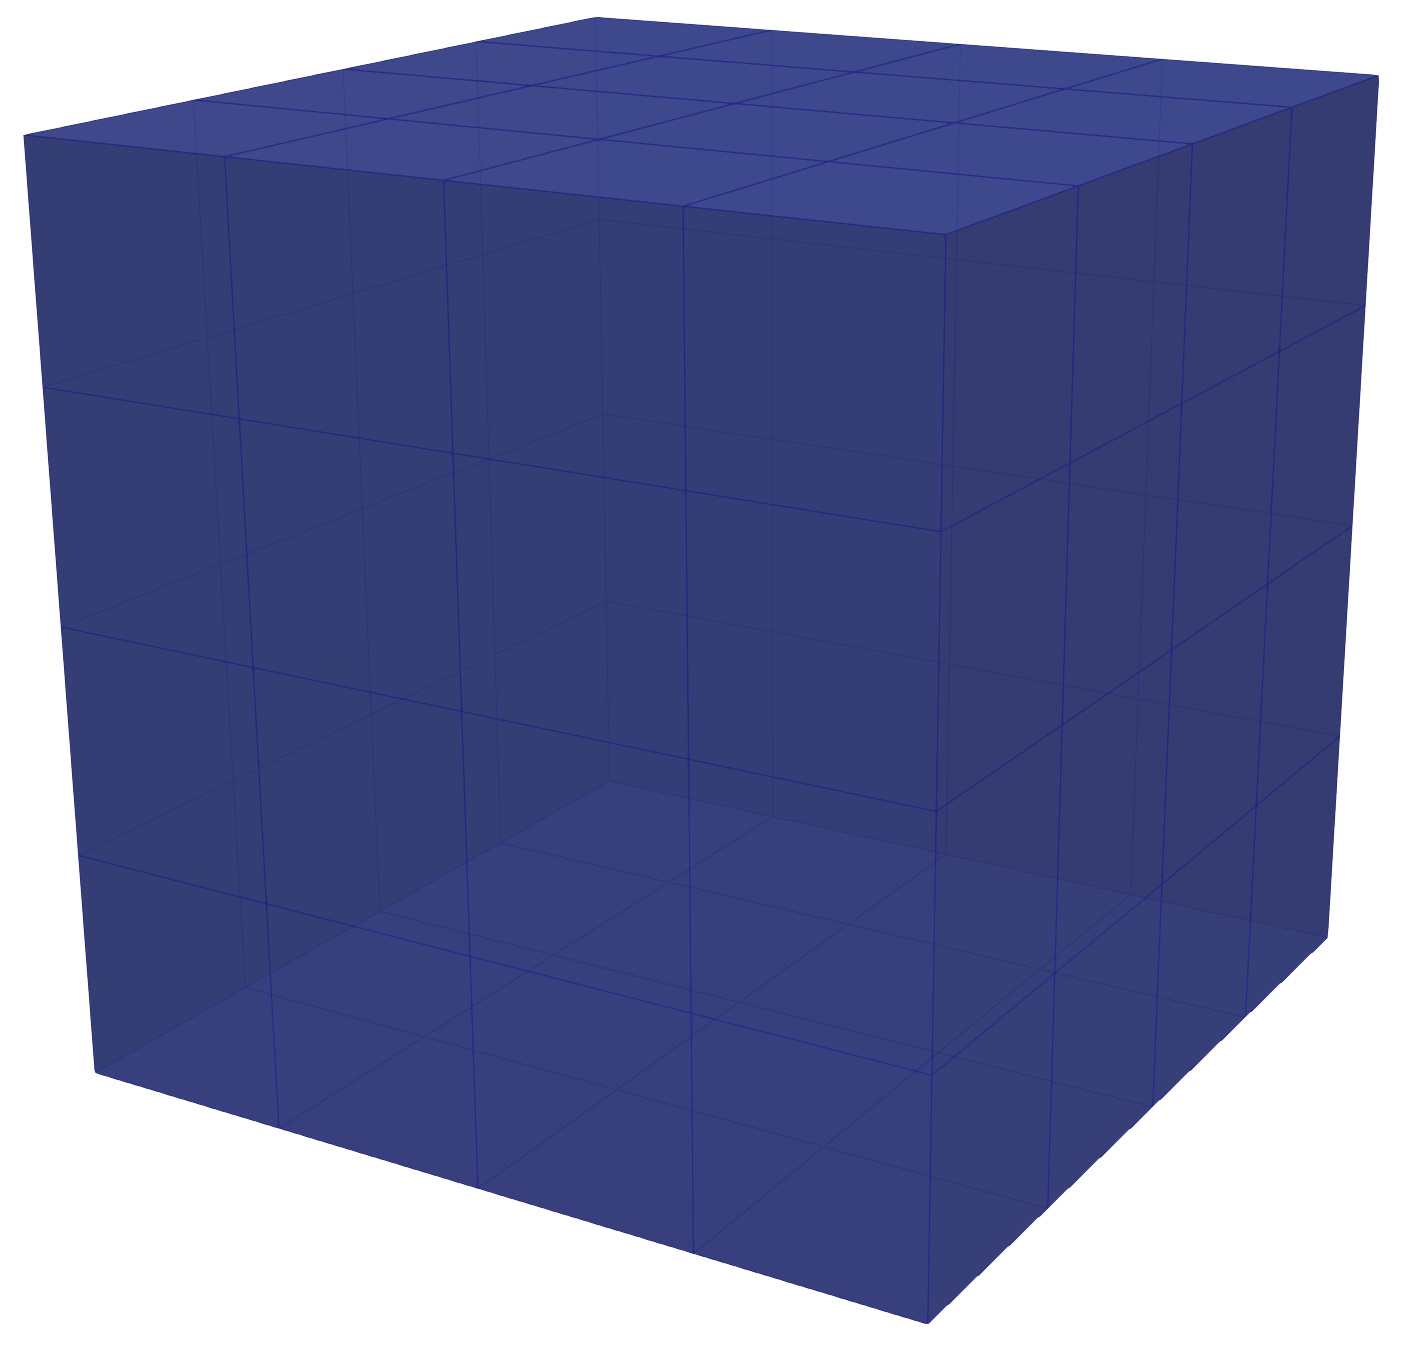
\includegraphics[width=\textwidth]{images/aac1.png}}
        \caption{Base source}
        \label{fig:aac1}
    \end{subfigure}
    \hfill
    \begin{subfigure}[b]{0.23\textwidth}
        \centering
        \raisebox{1.5cm}{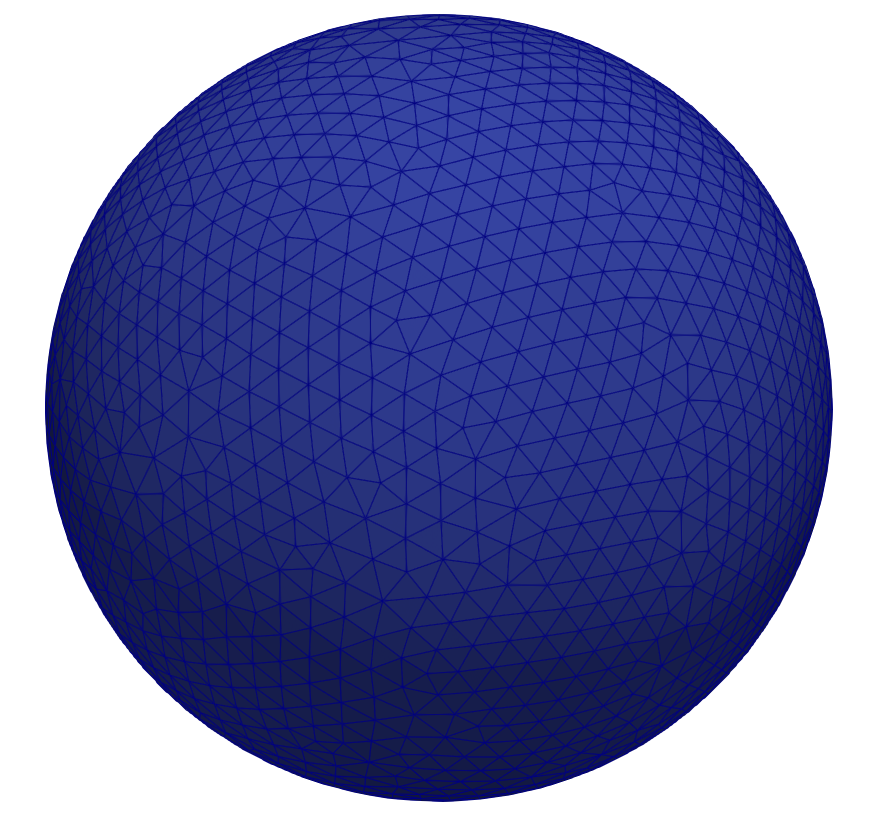
\includegraphics[width=\textwidth]{images/aac2.png}} % Adjust the 0.5cm value as needed
        \caption{Base cible}
        \label{fig:aac2}
    \end{subfigure}
    \hfill
    \begin{subfigure}[b]{0.35\textwidth}
        \centering
        \raisebox{0.0cm}{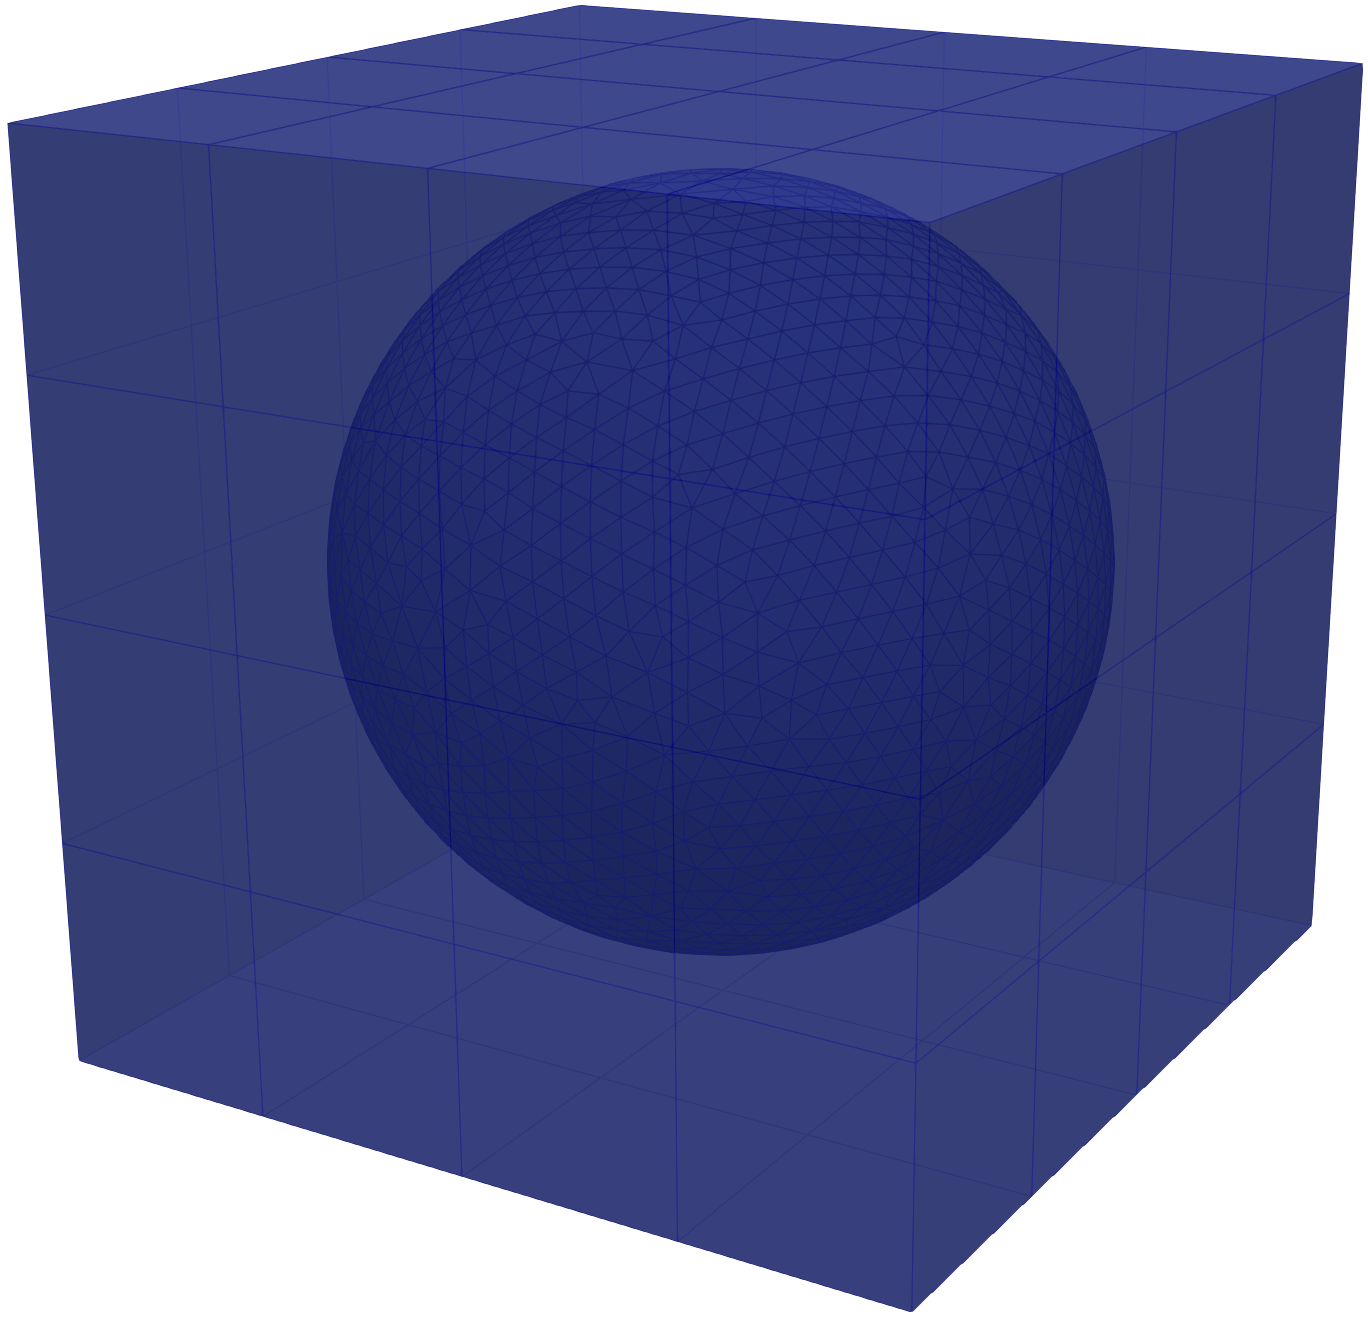
\includegraphics[width=\textwidth]{images/aac3.png}}
        \caption{Interpolation de la solution de la base source dans la base cible}
        \label{fig:aac3}
    \end{subfigure}
    \caption{Début de la chaîne aéroacoustique}
    \label{fig:composite}
\end{figure}



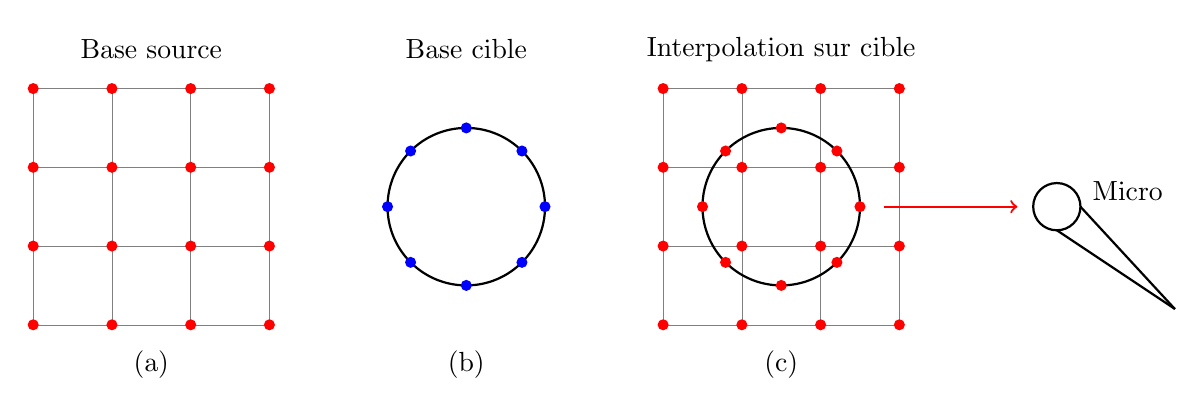
\begin{tikzpicture}

    % Step 1: Base source (rectangular grid)
    \draw[step=1cm,gray,very thin] (-3,0) grid (0,3);
    \node at (-1.5, 3.5) {Base source};
    \node at (-1.5, -0.5) {(a)};
    
    % Adding nodes and elements
    \foreach \x in {-3, -2, -1, 0} {
        \foreach \y in {0, 1, 2, 3} {
            \fill[red] (\x,\y) circle (2pt);
        }
    }
    
    %\node[anchor=west] at (0.2, 1.5) {$\sin(\text{pression})$};
    
    % Step 2: Base cible (circle)
    \draw[thick] (2.5,1.5) circle (1cm);
    \node at (2.5, 3.5) {Base cible};
    \node at (2.5, -0.5) {(b)};
    %\draw[->,thick,red] (2.5,1.5) -- (4, 1.5) node[midway,above] {Interpolation};

    % Discretize the circle with red points
    \foreach \angle in {0,45,...,315} {
        \fill[blue] ({2.5 + 1*cos(\angle)},{1.5 + 1*sin(\angle)}) circle (2pt);
    }
    
    % Step 3: Interpolated solution (target surface)
    \draw[step=1cm,gray,very thin] (5,0) grid (8,3);
    \draw[thick] (6.5,1.5) circle (1cm);
    \node at (6.5, 3.5) {Interpolation sur cible};

    \foreach \angle in {0,45,...,315} {
        \fill[red] ({6.5 + 1*cos(\angle)},{1.5 + 1*sin(\angle)}) circle (2pt);
    }

    \node at (6.5, -0.5) {(c)};
    
    % Step 4: Application of FWH equations
    %\draw[->,thick,red] (8.5,1.5) -- (10, 1.5) node[midway,above] {FWH};
    %\node at (11.5, 1.5) {Calcul du son à distance};
    
    % Additional nodes and elements for interpolated solution
    \foreach \x in {5,6,7,8} {
        \foreach \y in {0,1,2,3} {
            \fill[red] (\x,\y) circle (2pt);
        }
    }

    % Step 4: Application of FWH equations and the microphone
    \node at (10.9, 1.7) {Micro};
    \draw[thick] (10,1.5) circle (0.3cm); % Micro symbol
    \draw[thick] (10.3,1.5) -- (11.5,0.2); % Micro "handle"
    \draw[thick] (10.0,1.2) -- (11.5,0.2); % Micro "handle"
    \draw[->,thick,red] (7.8,1.5) -- (9.5, 1.5); % Arrow from circle to microphone

\end{tikzpicture}




La base source contient la pression aéroacoustique, d'une onde sinusoïdale dans un maillage grossier (différents types de cellules ont été testés). La base cible est une sphère d'où les équations de FWH seront ensuite appliquées. Finalement, voilà le résultat (Figure \ref{fig:onde_aac}) pour ces paramètres :

- observateur quelconque, car Mach égal à 0;

\vspace{-0,2cm}
- fréquence du signal aéroacoustique : 40 Hz;

\vspace{-0,2cm}
- nombre de points de la base source : 3x4 (pour 3D et 4 points par dimension);

\vspace{-0,2cm}
- types de cellules de la base source : hexaèdres;

\vspace{-0,2cm}
- paramètres \(N\) et \(p\) par défaut;

\vspace{-0,2cm}
- longueur de la base source : 7,20 m;

\vspace{-0,2cm}
- diamètre de la base cible : 6 m;

\vspace{-0,2cm}
- gamma = 1.4;

\vspace{-0,2cm}
- vitesse du son : 340.0 m/s;

\vspace{-0,2cm}
- masse volumique de l'air = 1.1825 kg/m3;

\vspace{-0,2cm}
- constante spécifique de l'air = 287.058 m2/(s2xK).
%- paramètres physiques : non énumérés, proches de ceux du \ac{SI}. 

\begin{figure}[H]
    \centering
    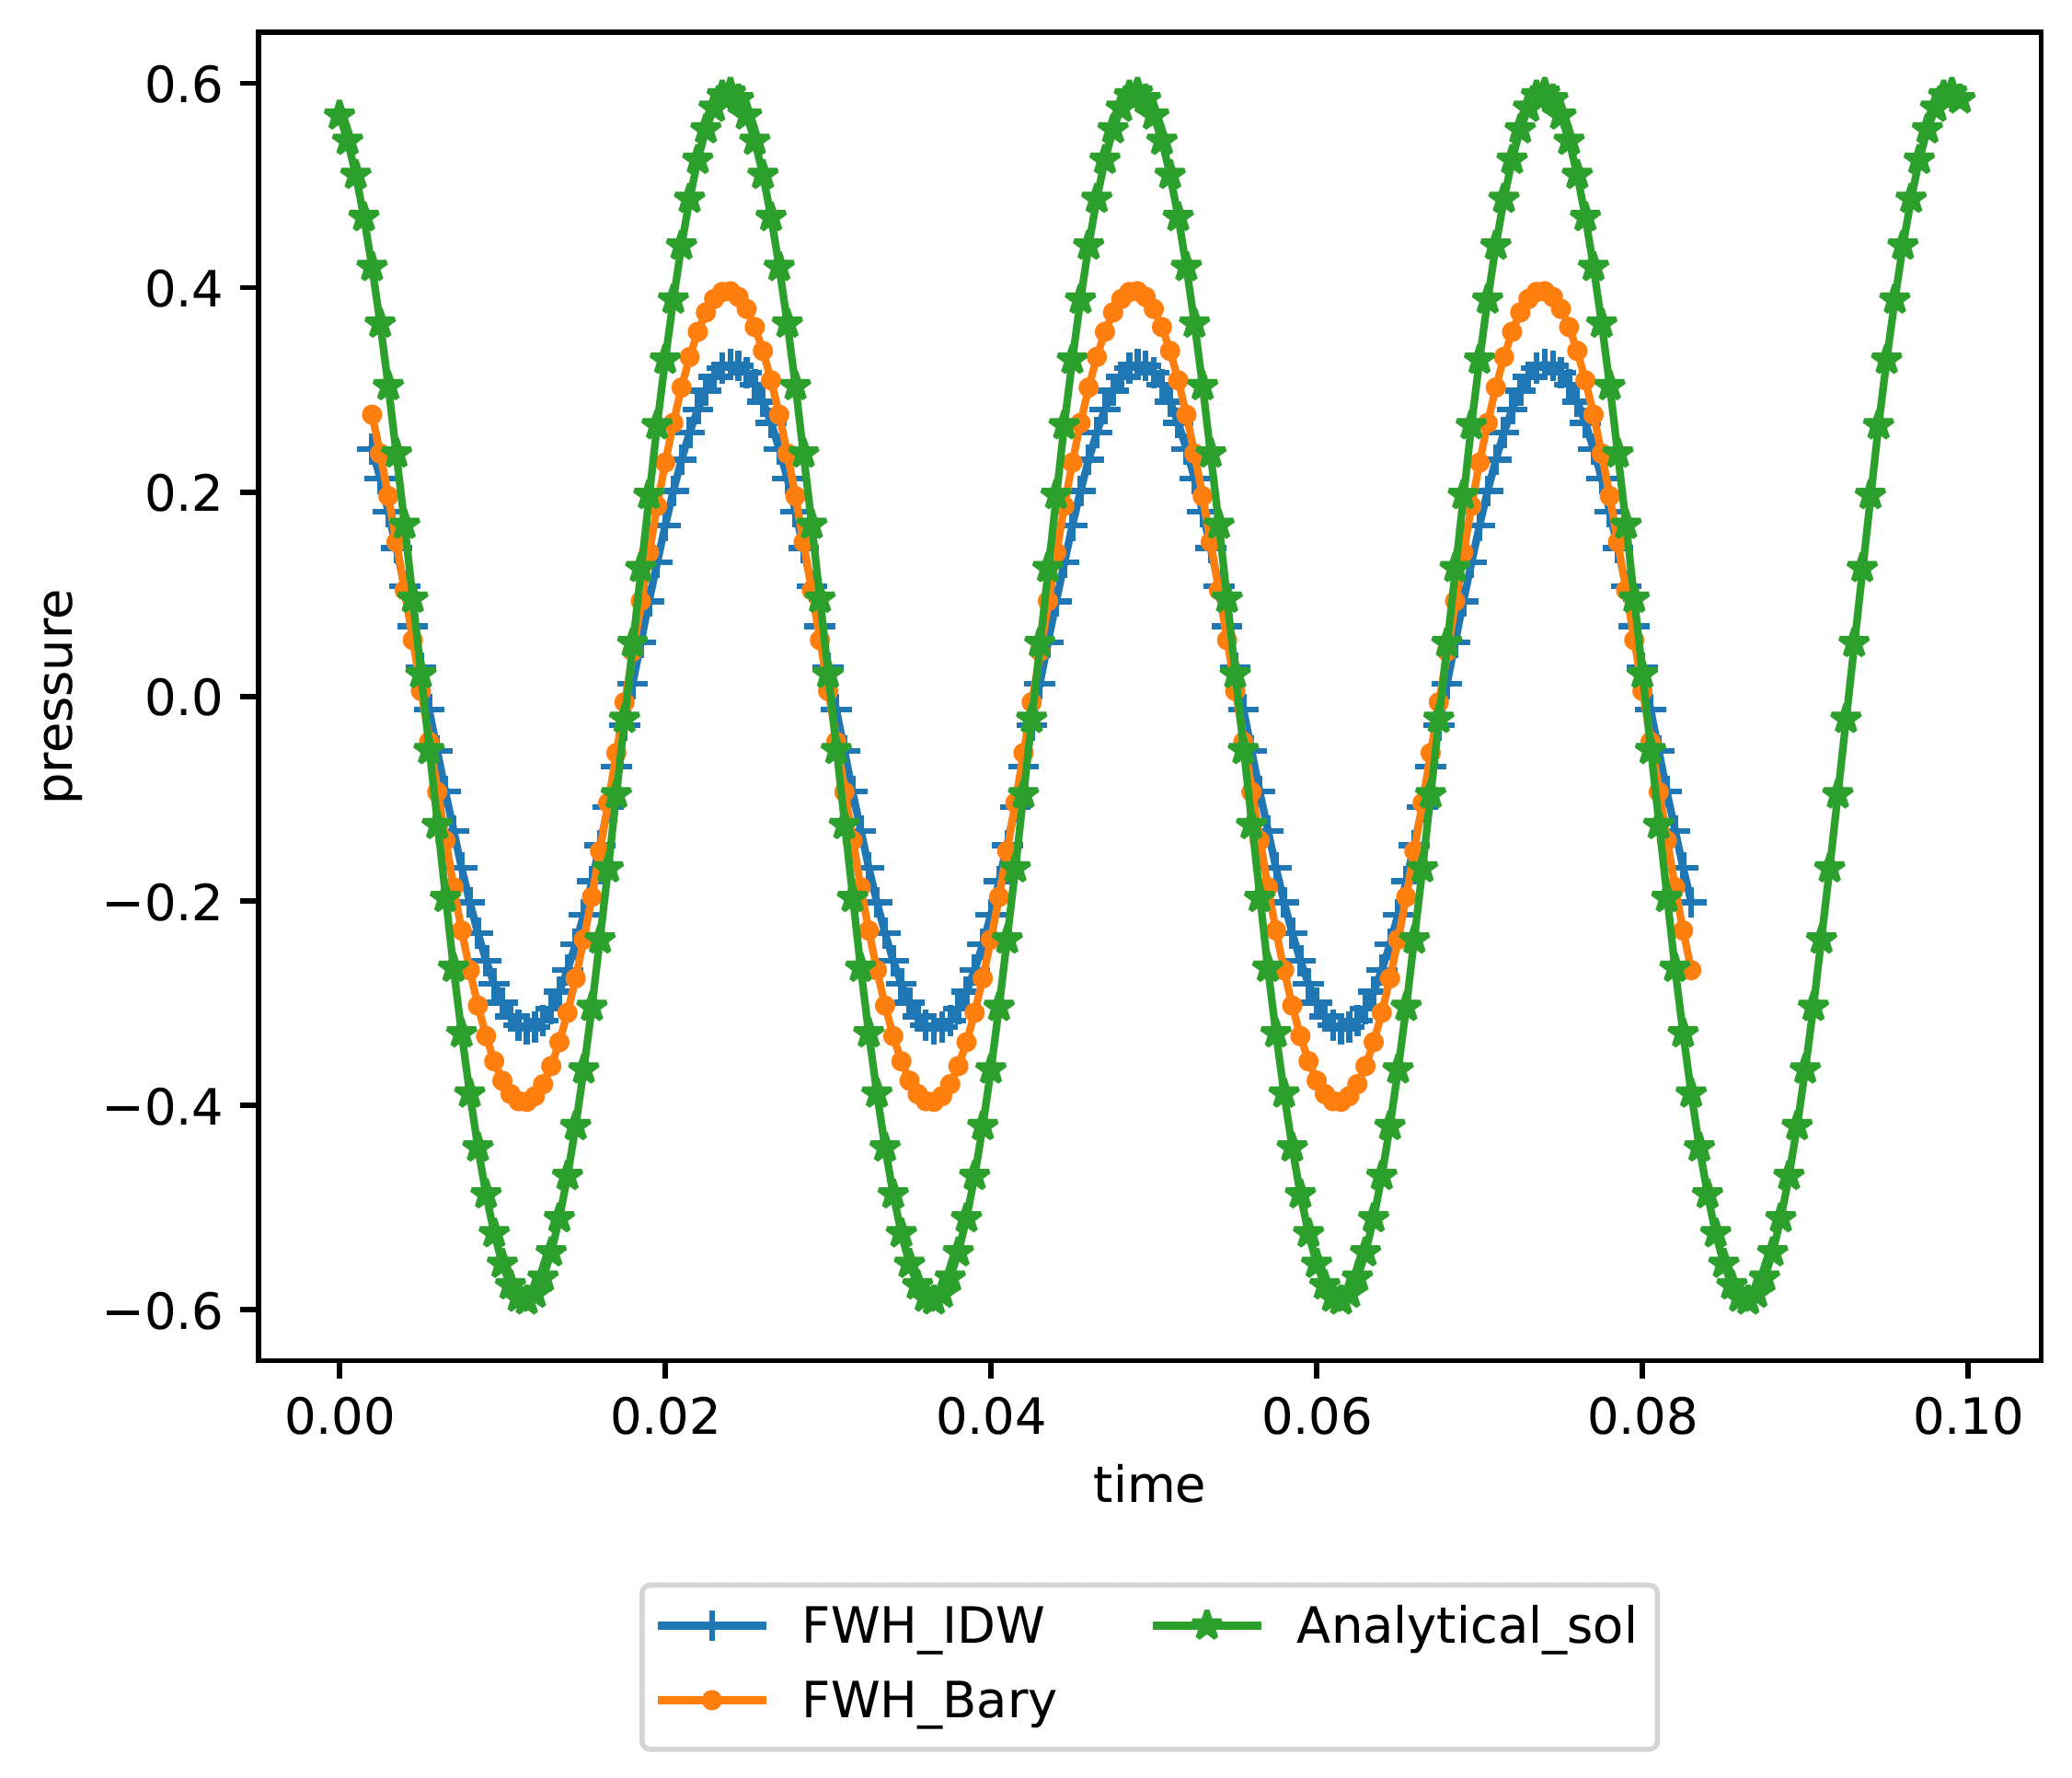
\includegraphics[width=0.67\textwidth]{images/onde_aac.png}
    \caption{Comparaison entre la solution analytique et la solution utilisant l'interpolation IDW et linéaire}
    \label{fig:onde_aac}
\end{figure}

L'erreur, au sens des moindres carrés, est plus élevée pour la méthode IDW que pour la méthode linéaire (ce qui est observable sur la Figure \ref{fig:onde_aac}).
Une amélioration possible de l'interpolation pour le cas de l'aéroacoustique serait d'utiliser la méthode d'interpolation par partie décrite dans des articles de l’ONERA \cite{cunha2011, cunha2016}
Pour des cas test et applications dédiés à l'aéronautique, il peut être intéressant de regarder les caractéristiques du bruit d'un avion, comme ses fréquences d'émission dans l'audible. \cite{frequence}

\subsection{Tests sur les paramètres de la méthode IDW}

La méthode IDW contient deux paramètres (\(N\) et \(p\)) dans son équation présentée dans la partie \ref{parametres}.

Pour savoir quels paramètres sont optimaux, des tests ont été menés sur le même cas que dans la sous-partie précédente, mais cette fois, ce qui nous intéresse est l'erreur au sens des moindres carrés, entre la solution analytique et IDW, en fonction des paramètres (\(N\) et \(p\)). Cette erreur est liée au rapport d'amplitude entre les deux courbes, ce qui a finalement été pris en compte. En les faisant varier, nous trouvons un minimum (local) pour \(N\)=10 et \(p\)=10 pour des paramètres similaires à la figure \ref{fig:onde_aac}.
Ces tests ont été menés sur kraken afin de ne pas perdre trop de temps.

\begin{figure}[H]
    \centering
    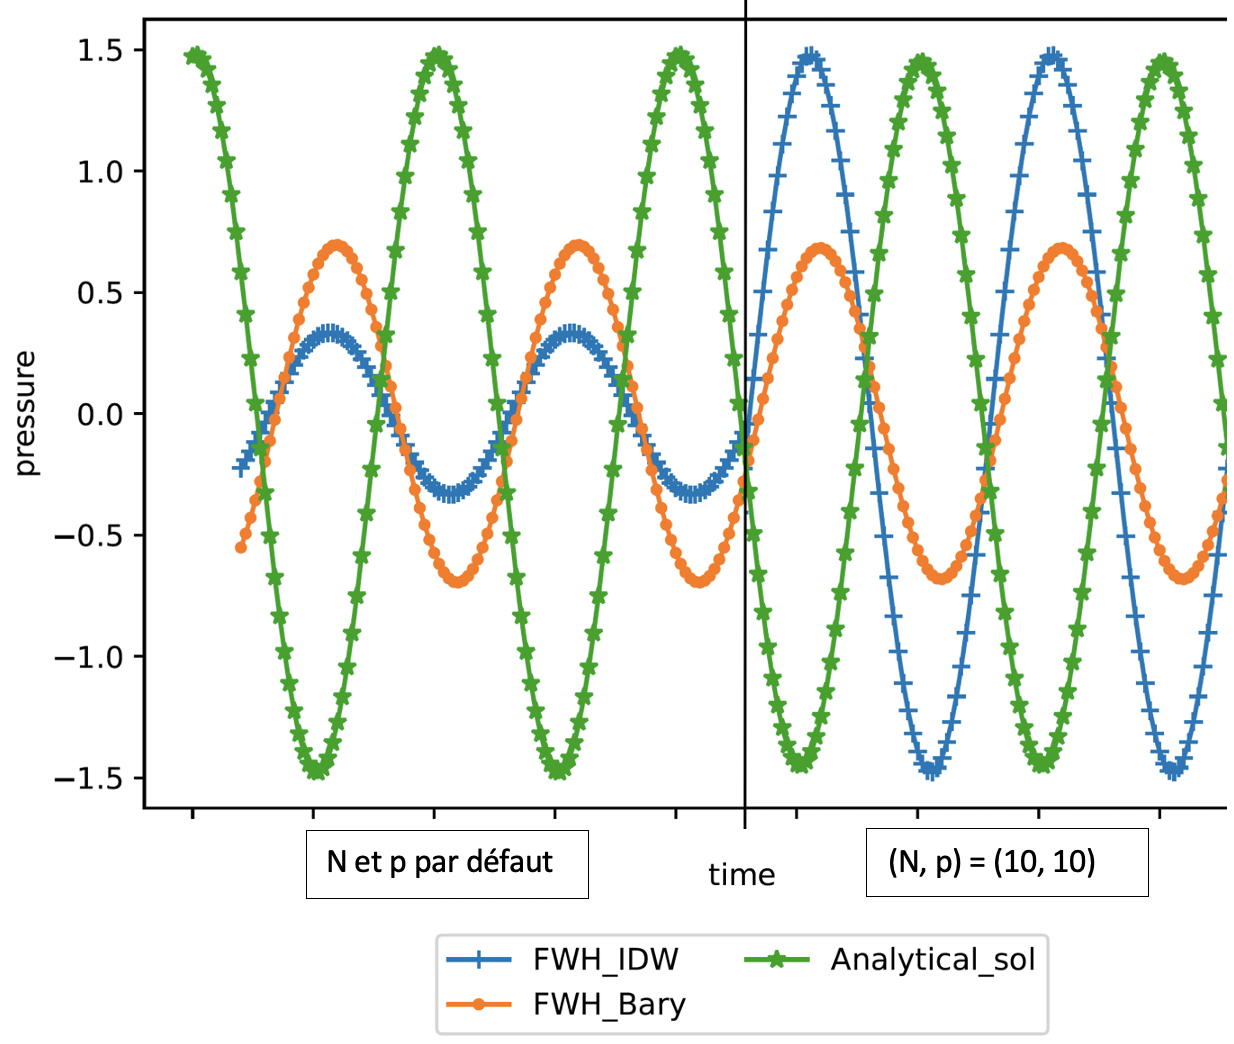
\includegraphics[width=0.70\textwidth]{images/rapport_a_np.png}
    \caption{Comparaison entre la solution analytique et la solution utilisant l'interpolation IDW (p=10, N=10) et linéaire}
    \label{fig:np10}
\end{figure}

À gauche, la méthode linéaire est utilisée, à droite la méthode IDW avec comme paramètres (N=10, p=10)(\ref{fig:np10}). Le décalage latéral des courbes est un artefact (et cela permet de mieux distinguer les courbes bleues et vertes dans notre cas.)
Le rapport d'amplitude avec la solution analytique est le suivant : idw = 102\%, linéaire = 48\%. Soit une erreur de 2\% pour idw et 52\% pour le linéaire. % pour dipole et quadripôle






